% VLDB template version of 2020-08-03 enhances the ACM template, version 1.7.0:
% https://www.acm.org/publications/proceedings-template
% The ACM Latex guide provides further information about the ACM template

\documentclass[sigconf, nonacm]{acmart}

\usepackage{amsmath}
\newtheorem{definition}{Definition}
\usepackage{bbding}
\usepackage{booktabs}
\usepackage{graphicx}
\usepackage{subcaption}
\usepackage{balance}
\usepackage{hyperref}
\usepackage{minted}
\usepackage[inline]{enumitem}
\usepackage{tikz}
\usetikzlibrary{arrows.meta}
\usepackage[linesnumbered,ruled,noend]{algorithm2e}
\SetKwInOut{Input}{input}\SetKwInOut{Output}{output}
\SetKwProg{Fn}{function}{}{end}
\SetKwSwitch{Match}{Case}{Other}{match}{do}{case}{otherwise}{endcase}

%% The following content must be adapted for the final version
% paper-specific
\newcommand\vldbdoi{XX.XX/XXX.XX}
\newcommand\vldbpages{XXX-XXX}
% issue-specific
\newcommand\vldbvolume{14}
\newcommand\vldbissue{1}
\newcommand\vldbyear{2021}
% should be fine as it is
\newcommand\vldbauthors{\authors}
\newcommand\vldbtitle{\shorttitle}
% leave empty if no availability url should be set
\newcommand\vldbavailabilityurl{http://vldb.org/pvldb/format_vol14.html}
% whether page numbers should be shown or not, use 'plain' for review versions, 'empty' for camera ready
\newcommand\vldbpagestyle{plain}

\begin{document}
\title{Out-of-Core Property Graph Matching for Real-World Graph Databases}

%%
%% The "author" command and its associated commands are used to define the authors and their affiliations.
\author{Yanxuan Cui}
\affiliation{%
  \institution{Tsinghua University}
  \city{Being}
  \state{China}
  \postcode{100084}
}
\email{cuiyx18@mails.tsinghua.edu.cn}

\begin{abstract}
  Property graph matching is the most important operation of graph database and has a wide range of applications.
  The problem has been studied extensively, however, on oversimplified graph models.
  Because of the complexity involving directions, multi-edges, labels in property graphs,
  optimizations aimed at simple graphs are not suitable to handle the storage and matching problem of property graphs.
  Moreover, existing approaches rely on huge memory resources to run their system and hinder the popularity of graph technology.

  We present SeqStar, the first out-of-core property graph matching system that can execute real-world complex queries efficiently.
  The storage engine of SeqStar uses a novel \emph{vertex-centric} storage model.
  By storing necessary information together with the vertices,
  SeqStar avoids the random disk access problem of existing work.
  In the graph matching engine, we propose a novel star decomposition algorithm that preserves all the relevant filtering information on stars.
  Therefore, SeqStar can filter out more unnecessary matchings in the very beginning.
  To reduce the memory usage, SeqStar compresses the intermediate results from star matching and performs pipeline join on the compressed data.
  Moreover, we propose a predicate pushdown method for SeqStar to optimize real-world queries.
\end{abstract}


\maketitle

%%% do not modify the following VLDB block %%
%%% VLDB block start %%%
\pagestyle{\vldbpagestyle}
\begingroup\small\noindent\raggedright\textbf{PVLDB Reference Format:}\\
\vldbauthors. \vldbtitle. PVLDB, \vldbvolume(\vldbissue): \vldbpages, \vldbyear.\\
\href{https://doi.org/\vldbdoi}{doi:\vldbdoi}
\endgroup
\begingroup
\renewcommand\thefootnote{}\footnote{\noindent
This work is licensed under the Creative Commons BY-NC-ND 4.0 International License. Visit \url{https://creativecommons.org/licenses/by-nc-nd/4.0/} to view a copy of this license. For any use beyond those covered by this license, obtain permission by emailing \href{mailto:info@vldb.org}{info@vldb.org}. Copyright is held by the owner/author\@(s). Publication rights licensed to the VLDB Endowment. \\
\raggedright{} Proceedings of the VLDB Endowment, Vol. \vldbvolume, No. \vldbissue\ %
ISSN 2150--8097. \\
\href{https://doi.org/\vldbdoi}{doi:\vldbdoi} \\
}\addtocounter{footnote}{-1}\endgroup
%%% VLDB block end %%%

%%% do not modify the following VLDB block %%
%%% VLDB block start %%%
\ifdefempty{\vldbavailabilityurl}{}{
\vspace{.3cm}
\begingroup\small\noindent\raggedright\textbf{PVLDB Artifact Availability:}\\
The source code, data, and/or other artifacts have been made available at \url{\vldbavailabilityurl}.
\endgroup
}
%%% VLDB block end %%%
\section{Introduction}
Graph matching
%~\footnote{There are two kinds of graphs in a graph matching problem: one is the large \emph{data graph}, the other is the much smaller \emph{pattern graph}}
is one of the most important applications of graph databases. In graph matching, a relative small \emph{pattern graph} is used to match subgraphs of a relative large \emph{data graph}.
It is widely used in many fields,
such as Twitter's recommendation systems~\cite{DBLP:journals/pvldb/GuptaSGGZLL14,DBLP:journals/pvldb/SharmaJBLL16},
electronic computer-aided design~\cite{DBLP:conf/dac/OhlrichEGS93},
and protein-protein interaction (PPI) networks~\cite{milenkovic2008uncovering}.
Nowadays, users of industrial graph databases such as Neo4j\footnote{\url{https://neo4j.com}}
can easily model data as property graphs and expressing their queries via the Cypher~\cite{DBLP:conf/sigmod/FrancisGGLLMPRS18} query language.
Although it is convenient to use, the matching process of these industrial graph databases are time and resource consuming.
Many novel subgraph matching algorithms have been proposed~\cite{DBLP:journals/pvldb/SunWWSL12,DBLP:conf/sigmod/HanLL13,DBLP:conf/sigmod/ShaoCCMYX14,DBLP:conf/cloud/SerafiniMS17,DBLP:journals/pvldb/QiaoZC17,DBLP:conf/sigmod/DiasTGM019}, with even orders of magnitude of speedup compared to the industrial graph databases.
However, there are two gaps that hinder these algorithms from being widely adopted in the real-world scenarios:
(1) the gap between the complexity of real-world queries and the simplicity of graphs that the existing algorithms can handle;
(2) the huge memory and high-speed network requirements for the existing algorithms to query on large graphs and the limitation of resource budget.

The property graph is the de facto graph model for real-world graph matching problems.
A property graph is a directed graph with labels attached to vertices and edges.
There may be multiple edges connecting two vertices and even edges for self-loop (edges connecting back to their source vertices).
Moreover, users usually provide extra searching conditions via the WHERE clause~\cite{DBLP:journals/csur/AnglesABHRV17}. However,  current studies mostly deal with simple graph models such as ignoring the directions, labels, or multi-edges. WHERE clause is not considered either~\cite{DBLP:journals/pvldb/SunWWSL12,DBLP:conf/sigmod/HanLL13,DBLP:conf/sigmod/KimLBHLKJ16,DBLP:journals/pvldb/QiaoZC17,DBLP:journals/pvldb/MhedhbiS19}. The optimizations aimed at simple graphs usually heavily rely on the equivalence of vertices~\cite{DBLP:conf/sigmod/HanLL13,DBLP:journals/pvldb/QiaoZC17}, which is harder to find in a property graph because of the complexity of directions and labels. Moreover, in the implementation level, the storage engine designed for simple graph models encounters excessive random disk seeks when matching a real-world property graph.

%This limitation is not only a matter of engineering,
%but also a serious algorithm problem:
%(1) the storage engine designed for simple graph may encounter superfluous random disk reads when matching a property graph;
%(2) the optimizations aimed at simple graph usually rely heavily on the equivalence of vertices~\cite{DBLP:conf/sigmod/HanLL13,DBLP:journals/pvldb/QiaoZC17}, which is harder to find in a property graph because of the complexity of directions and labels.

Existing algorithms rely on main memory for their computation. It is extremely uneconomic for property graph matching problem. The memory needs to hold not only the graph data but also the intermediate results which grow exponentially with respect to the size of graph data. Our experiment shows that a graph with $6.9 \times 10^{7}$ edges could generate $1.7 \times 10^{13}$ rows of matching results.
%(1) The memory needs to hold not only the data graph, but also the intermediate result which grows exponentially with respect to the size of the data graph, as our experiment shows that a graph with $6.9 \times 10^{7}$ edges could generate $1.7 \times 10^{13}$ rows of matching results.
Existing systems~\cite{DBLP:conf/sosp/TeixeiraFSSZA15,DBLP:conf/sigmod/DiasTGM019,DBLP:journals/pvldb/MhedhbiS19} require hundreds of GB of memory to process such graphs. Therefore, we resort to use external memory (such as SSDs) to support property graph matching.
%(2) For distributed approaches, on the one hand it is hard to partition the graph across cluster machines to minimize the communication cost~\cite{DBLP:journals/im/LeskovecLDM09} and have performance problems~\cite{DBLP:conf/sigmod/KimLBHLKJ16},
%one the other hand it is inconvenient and costly for the end user to maintain the cluster nodes~\cite{DBLP:conf/osdi/KyrolaBG12}.

This paper proposes SeqStar, a high performance out-of-core property graph matching system for real-world graphs, which scans the disk sequentially by matching stars (a star contains a root vertex and some leaves which are the neighbors of the root).

%Therefore, in order to match up with the need of real-world problems,a high performance disk-based property graph matching system is desirable.

\subsection*{Contributions}
There are two fundamental components in SeqStar:
the graph storage engine and the graph matching engine. Both are designed specificly to deal with the graph machine problem efficiently.

The storage engine in SeqStar uses the \emph{vertex-centric storage model} which stores the information related to a specific vertex together.
The conventional way to store graphs is the compressed sparse row (CSR) and compressed sparse column (CSC) approach which stores in/out-edges \emph{separately}~\cite{DBLP:conf/sc/PearceGA10,DBLP:conf/osdi/KyrolaBG12}.
CSR is equivalent to storing the graph as adjacency list: the out-edges are stored consecutively on disk.
And CSC stores the in-edges in a similar manner.
In contrast, SeqStar stores the graph data by storing the in/out-edges \emph{together} with the neighbors of each vertex.
With small indexes on disks, pattern matching can quickly get the correct address of relevant data on disk during pattern matching.
We also provide two convenient iterator interfaces to interact with the storage engine.
As a result, SeqStar can avoid random disk seeks and perform graph matching in a sequential disk scan.

For the graph matching engine, SeqStar uses a star decomposition based algorithm to run graph matching.
The analyzer of SeqStar analyzes the graph matching query and select a vertex-cover heuristically as the roots of stars.
%这里加一句如何把原图分解为星型子图
We save all useful filtering information in each star subgraph after decomposition. To reduce the amount of memory that would be used as the storage of intermediate results, a novel compression method, which postponing Cartesian production and digging equivalence classes, is used for star matching results. SeqStar's efficient and scalable pipeline join algorithm is able to process the compressed data. To the best of our knowledge, SeqStar is the first system that integrates the optimization of WHERE clauses in the graph matching algorithm, by pushing the predicates down to the star matching process.

According to our experiments, SeqStar outperforms the state-of-the-art graph querying system Graphflow by up to $26\times$.
And SeqStar can run the queries that Graphflow fails to run due to the out of memory problem.
For complex property graphs that existing academic researches do not support,
we compare SeqStar with industrial graph database Neo4j, and achieved over $2100\times$ speedup.
%To reduce memory usage, we make the following contributions:
%(1) a novel star decomposition algorithm that keeps all the useful filtering information in stars,
%(2) a novel compression algorithm for stars' matching results by postponing Cartesian production and digging equivalence classes,
%(3) an efficient and scalable pipeline join algorithm that is able to process the compressed data directly.

%Moreover, to the best of our knowledge, we are the first one to integrate the optimization of WHERE clauses in the graph matching algorithm, by pushing the predicates down to the star matching process.
%% The conventional graph storage method is the compressed sparse column (CSC) and the compressed sparse row (CSR) format~\cite{DBLP:conf/osdi/KyrolaBG12},
%% which stores the in/out-edges separately for each vertex.
%% However, because of the multi-edges in property graphs, the in/out-edges have to be searched many times to check the matching of a vertex, and result in excessive random disk seeks.
%% To address this challenge, we propose the \emph{vertex-centric storage model} that stores all the necessary information together with the vertices, such that the vertices could be matched in a single sequential scan.

%% Generally speaking, there are two kinds of graph isomorphism algorithm,
%% differing on whether intermediate results are materialized.
%% The first is the backtracking tree-searching method~\cite{DBLP:journals/jacm/Ullmann76,DBLP:journals/pvldb/LeeHKL12,DBLP:conf/sigmod/HanLL13,DBLP:conf/sigmod/KimLBHLKJ16},
%% which does not generate intermediate results but have scaling problems~\cite{DBLP:conf/cloud/SerafiniMS17}.
%% The second is the join-based algorithm~\cite{DBLP:journals/pvldb/LaiQLC15,DBLP:journals/pvldb/QiaoZC17,DBLP:journals/pvldb/SunWWSL12,DBLP:journals/pvldb/MhedhbiS19},
%% which decomposes the pattern graph into smaller matching unit and materialize the intermediate results,
%% and the final result is obtained by joining on these intermediate results.
%% Because of the notorious poor locality of graphs,
%% enormous amount of random disk accesses would be encountered for an out-of-core tree-searching approach.
%% Based on this observation, this paper designs a join-based property graph matching algorithm.

%% The most fundamental problem of a graph matching algorithm is to determine the basic matching unit.
%% Edges are the simplest matching units, however, intermediate results much larger than the data graph would be generated and result in costly join operations.
%% To avoid excessive joins, authors use more complex structures i.e.,
%% frequent subgraphs, multi-hop edges, or cliques as their matching unit~\cite{DBLP:conf/sigmod/HeS08,DBLP:conf/edbt/ZhangLY09,DBLP:journals/pvldb/QiaoZC17}, however,
%% these algorithms rely on super-linear indices~\cite{DBLP:journals/pvldb/SunWWSL12}.
%% To address this challenge, we make a balance by choosing stars as our basic unit.
%% And our star decomposition algorithm is enhanced such that the stars keep as much filtering information as possible.
%% Our experiment shows that this enhancement could reduce the intermediate results by up to $43\%$ of the existing works.

%% However, the stars' matching results could still be very large because the matching results grow exponentially with respect to the data graph,
%% e.g., a 129M graph could easily eat up hundreds or even thousands GB of memory to store the intermediate results.
%% Inspired by VCBC~\cite{DBLP:journals/pvldb/QiaoZC17}, we develop a novel compression algorithm for star' matching result by postponing the costly Cartesian product and digging the equivalence classes in the leaves of the star.
%% The compression ratio is quite impressive, as high as $10^8$,
%% and we find that the size of the compressed star's matching results takes less than $23\%$ the space to store the graph,
%% which can even fit into the main memory of a laptop.

\section{Background}\label{sec:background}
This section introduces the formal definition of property graphs, and then discusses the property graph matching problem.
\subsection{Property Graph Model}
A \emph{property graph} is a directed vertex-labeled edge-labeled multigraph with self-edges,
and key-value properties are stored on vertices and edges.
We now provide the formal definition of a property graph.
\begin{definition}[Property Graph~\cite{DBLP:journals/csur/AnglesABHRV17}]
  A property graph $G$ is a tuple $(V, E, \rho, \lambda, \sigma)$, where:
  \begin{enumerate}[noitemsep,label={(\arabic*)}]
  \item $V$ is a finite set of vertices.
  \item $E$ is a finite set of edges such that $V$ and $E$ have no elements in common.
  \item $\rho: E \rightarrow (V \times V)$ is a total function.
    Intuitively, $\rho(e) = (v_1, v_2)$ indicates that $e$ is a directed edge from $v_1$ to $v_2$.
  \item $\lambda :(V \cup E) \rightarrow L$ is a total function where $L$ is a set of labels.
    Intuitively, if $v \in V, \rho(v) = l$ (respectively, $e \in E, \rho(e) = l$),
    then $l$ is the label of vertex $v$ (respectively, edge $e$).
  \item $\sigma: (V \cup E) \times Prop \rightarrow Val$ is a partial function with $Prop$ a finite set of properties and $Val$ a set of values.
    Intuitively, if $v \in V, p \in Prop, \sigma(v, p) = s$ (respectively, $e \in E, p \in Prop, \sigma(e, p) = s$),
    then $s$ is the value of property $p$ for vertex $v$ (respectively, edge $e$) in the property graph $G$.
  \end{enumerate}
\end{definition}
For simplicity, in this paper, we do not discuss the properties i.e., $\sigma$ in $G$,
because similar techniques can be used as processing the labels $\lambda$.
Thus, the property graph $G$ can be denoted by $(V(G), E(G), \rho_G, \lambda_G)$.
Please note that the total function $\rho_G$ is necessary, in general,
we cannot identify an edge simply by the starting and ending vertices such as $(u_1, u_2)$ as can be done in the simple graph model,
because multiple edges may appear between the two vertices.
However, we may use the $(u_1, u_2)$ notation if all we care about is that there exist at least one edge between $u_1$ and $u_2$.
\begin{definition}[Vertex Cover]
  A vertex cover $V_c$ of a property graph $G$ is a subset of $V(G)$ such that
  $\forall e \in E(G), \rho_G(e) = (u, v) \implies u \in V_C \lor v \in V_C$.
\end{definition}
\subsection{Property Graph Matching Problem}
\begin{definition}[Subgraph]
  A property graph $F$ is called a subgraph of a property graph $G$, written $F \subseteq G$, if
  $V(F) \subseteq V(G)$, $E(F) \subseteq E(G)$, $\rho_F$ is a restriction of $\rho_G$, and $\lambda_F$ is a restriction of $\lambda_G$.
\end{definition}
Let $G$ be any property graph, and let $S \subseteq V(G)$, then the \emph{induced subgraph} $G[S]$ is the graph whose vertex set is $S$ and whose edge set consists of all of the edges in $E(G)$ that have both endpoints in $S$.
\begin{definition}[Property Graph Isomorphism]
  Two property graphs $G$ and $H$ are isomorphic, written $G \cong H$,
  if there exists bijections $\theta: V(G) \rightarrow V(H)$ and $\phi: E(G) \rightarrow E(H)$ such that
  $\rho_G(e) = (u, v)$ if and only if $\rho_H(\phi(e)) = (\theta(u), \theta(v))$,
  $\lambda_G(v) = \lambda_H(\theta(v))$ for all $v \in V(G)$
  and $\lambda_G(e) = \lambda_H(\phi(e))$ for all $e \in E(G)$;
  Such a pair of mappings is called an isomorphism between $G$ and $H$.
\end{definition}
The bijection $\theta: V(G) \rightarrow V(H)$ is the key in the definition of property graph isomorphism,
because the bijection $\phi: E(G) \rightarrow E(H)$ is straightforward if $\theta$ is fixed.
However, due to automorphism, where an \emph{automorphism} of a graph is an isomorphism of the graph to itself,
the bijection $\theta$ may not be unique.
\begin{definition}[Property Graph Matching]\label{def:property_graph_matching}
  Given a data property graph $D$, a pattern property graph $P$ and a searching condition $\psi: PG \rightarrow B$ with $PG$ the set of property graph and $B$ the set of Boolean values,
  the property graph matching problem is to report the set $\mathcal{I} = \{F | F \subseteq D, F \cong P, \psi(F) = true\}$.
\end{definition}
Authors of previous works usually omit the searching condition $\psi$ in their definition of graph matching~\cite{DBLP:conf/sigmod/ShaoCCMYX14,DBLP:journals/pvldb/LaiQLC15,DBLP:conf/sigmod/KimLBHLKJ16,DBLP:journals/pvldb/QiaoZC17}.
And they adopt a loosely related technique called \emph{symmetry-breaking}~\cite{DBLP:conf/recomb/GrochowK07},
which ensures there is a unique bijection $\theta: V(P) \rightarrow V(F)$ by providing a partial order on $V(P)$ after exploiting the automorphism of $P$.
However, as we have stated before, the WHERE clause is a ubiquitous part of the query language of a graph database.
Users of a real-world graph database usually provide their self-defined searching condition $\psi$ to filter out unnecessary matchings not only symmetry-breaking conditions.
Thus, the searching condition we defined here can be viewed as a super set of symmetry-breaking.
We add the searching condition in the definition because it is actually a part of the property graph matching problem,
and we also found that it can be decomposed and pushed down to lower phase to boost the evaluation of graph matching (Section~\ref{sec:framework}).

A property graph is always directed.
However, in some cases such as friendship, there is no need to pay attention to the directions of the edges.
In order to support this kind of relationship, a naive approach is to add a duplicate edge in opposite direction for each edge in the data graph.
More elegantly, we allow the pattern graph $P$ to contain undirected edges.
Users can simply ignore the direction by providing undirected edges in $P$ like in industrial graph databases such as Neo4j.

\section{Overview of SeqStar}\label{sec:framework}
We demonstrate the workflow of SeqStar in this section,
and use an example to show the query processing stages.
\subsection{SeqStar Workflow}
\begin{figure}[ht]
  \centering
  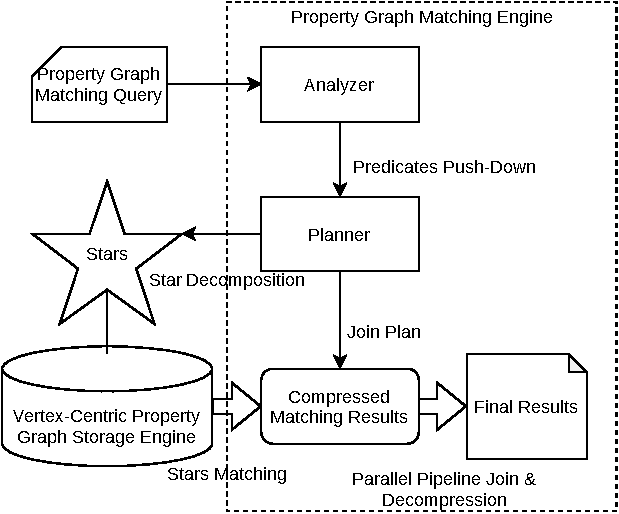
\includegraphics[width=0.48\textwidth]{img/architecture.pdf}
  \caption{SeqStar workflow.}\label{img:architecture}
\end{figure}
Figure~\ref{img:architecture} shows the workflow of SeqStar. There are mainly two building blocks in SeqStar: the storage engine and the property graph matching engine.
Both are specially designed to deal with the property graph matching problem efficiently.

Traditional graph storage engines such as used in graph databases store the in-edges and out-edges separately for each vertex.
Because of the complexity in property graphs,
such a storage method is not suitable and would incur many unnecessary random disk accesses.
We develop a vertex-centric property storage model to store all information related to one vertex together to address the problem (\S\ref{sec:storage}).


Based on the storage model,
we propose an efficient property graph matching engine that is able to execute real-world complex queries (\S\ref{sec:match}).
The core of the graph matching engine is the planner, which  decomposes the pattern into a series of stars.
Compared with existing works, we take a step further by introducing
(1) a matching result compression algorithm which reduces the cost of materializing intermediate results,
(2) a predicate pushdown optimizer that is able to filter out unnecessary matchings in early stages and mitigate the burden of the join process.
\subsection{Query Processing Stages}
Here is an example of how a concrete query gets executed in SeqStar.
Consider the Cypher (Neo4j's graph query language) query in Figure~\ref{img:cypher_query},
which generates the pattern graph in Figure~\ref{img:running_example} (b):

\begin{figure}[ht]
  \begin{Verbatim}[fontsize=\small]
    MATCH (u1:Person)-[:FOLLOWS]->(u2:Person)-[:FOLLOWS]->(u1),
          (u1)-[:FOLLOWS]->(u3:Person)-[:FOLLOWS]->(u1),
          (u1)-[:REPOSTS]->(u4:Media),
          (u2)-[:LIKES]->(u4)<-[:LIKES]-(u3)
    WHERE u2 > u1 AND NOT (u3 <= u1 OR u4 >= 8)
  \end{Verbatim}
  \caption{Example query.}\label{img:cypher_query}
\end{figure}

\begin{figure*}[ht]
  \centering
  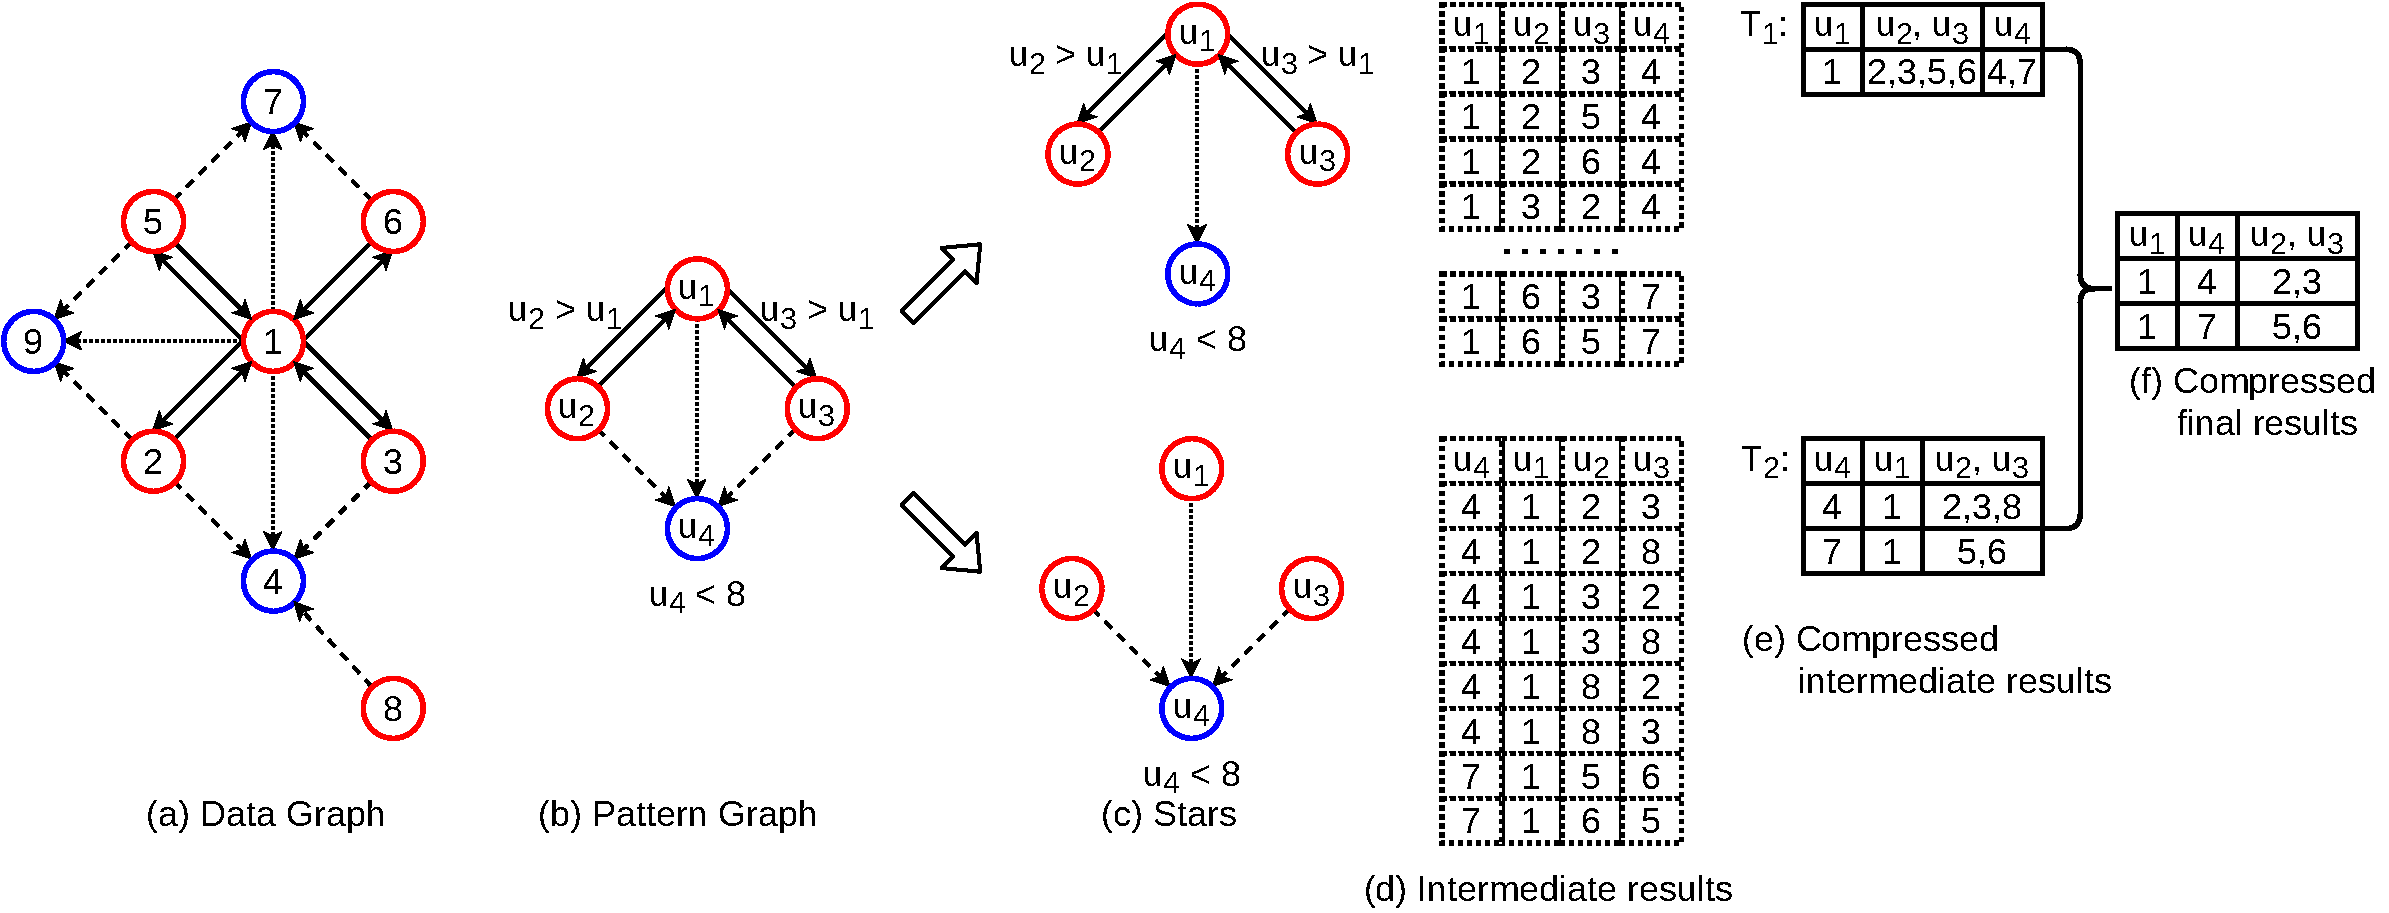
\includegraphics[width=\textwidth]{img/running_example.pdf}
  \caption{Working stages of the example query.}\label{img:running_example}
\end{figure*}

The analyzer firstly analyzes the WHERE clause and extract useful filtering information for early stage filtering.
SeqStar rewrites the WHERE clause to AND-separated expressions `$u_2 > u_1$ AND $u_3 > u_1$ AND $u_4 < 8$' by applying De Morgan's law.
The searching conditions $u_2> u_1$, $u_3 > u_1$ and $u_4 < 8$ are then attached to the pattern graph (Figure~\ref{img:running_example} (b)).
Based on the analysis result and the statistical information of the data graph,
the planner dynamiclly selects a connected vertex cover ($u_1, u_4$) in the pattern as the roots of stars.
The star generating algorithm keeps all the relevant edges and additional searching conditions in order to filter out unnecessary matchings as early as possible.

With the help of SeqStar's vertex-centric storage engine,
all the stars can be matched by only one sequential scan on the data graph (\S\ref{sec:match_star}).
For example, to match star $S_2$,
SeqStar seeks to the vertices labeled with ``Media'' (colored in blue) quickly by searching the index in the storage engine.
The candidate vertices $4, 7, 9, 10$ (vertices are identified by their IDs in integers) may match the root $u_4$.
Then SeqStar scans the candidate vertices sequentially and finds that only vertex $4, 7$ can be matched (vertex $9$ and $10$ violate the constraint $u_4 < 8$).

The intermediate results from star matching are not stored as conventional flat and incarnated rows. Instead, SeqStar compresses the intermediate results and uses pipeline joins without incarnation of some intermediate rows.

SeqStar compresses the intermediate results by digging equivalence classes among vertices and postponing Cartesian product to reduce memory usage (\S\ref{sec:match_compress}).
In the decomposed stars, $u_2$ and $u_3$ have the same label, and they also have the same connections to the root $u_1$ or $u_4$ ($u_2 > u_1$ and $u_3 > u_1$ are equivalent in this case because they both represent the filter $f(x): x > u_1$).
We say that $u_2$ and $u_3$ both belong to the same \emph{neighbor equivalence class}.
For each neighbor equivalence class, the matched vertices are stored together as an \emph{image set}.
For example $\{2, 3, 5, 6\}$ in $T_1$ is the image set of $u_2$ and $u_3$.
An \emph{image set} is the basic structure to hold the intermediate results.
While scanning each vertex $v$ in the data graph,
SeqStar checks the neighbors of $v$ and stores the matched neighbors together as image sets.
To match the star $S_2$,
for each candidate e.g., vertex $4$, SeqStar scans the neighbors of vertex $4$ and finds that $u_1$'s image set is $\{1\}$,
the image set of $u_2, u_3$ is $\{2, 3, 8\}$.
The tuple $(4, \{1\}, \{2, 3, 8\})$ is then appended to the compressed intermediate results, as a \emph{SuperRow}.
Note that the first column contains only one vertex, which matches the root of a star.

Finally, SeqStar performs the joins on SuperRows to obtain the final results (\S\ref{sec:match_join}) without the incarnation of intermediate rows. The planner generates a join order ($T_1 \Join T_2$ in this case) based on the statistical information of the SuperRows.
For each SuperRow $R_1$ in $T_1$, SeqStar scans the image set of $u_4$ and finds the corresponding SuperRow $R_2$ in $T_2$.
The join result of $u_2$, $u_3$ is obtained by the intersection if the corresponding columns of $R_1$ and $R_2$,
i.e., $\{2, 3, 5, 6\} \cap \{2, 3, 8\} = \{2, 3\}$, $\{2, 3, 5, 6\} \cap \{5, 6\} = \{5, 6\}$.
If more than two stars are decomposed from the pattern graph,
instead of join them one by one,
the planner in SeqStar will generate a pipeline plan to multi-join on the SuperRows.
By doing so, no new intermediate rows will be generated.
SeqStar generates the compressed final results in a stream manner.
The decompression by Cartesian product to get the final results is not performed     unless required. The compression and pipeline joining can efficiently reduce the memory consumption during computation.

%and the decompression is done by doing Cartesian production on the fly to report the final answer.

%% The vertex-centric storage engine is designed to be I/O efficient and support the real-world property graph well.
%% The conventional way to store graphs on disk is to store the in/out-edges separately for each vertex,
%% via the compressed sparse column (CSC) and the compressed sparse row (CSR) format~\cite{DBLP:conf/sc/PearceGA10}.
%% However, we find that the conventional graph storing method has limitations for real-world property graph:
%% because of the existence of multi-edges,
%% one has to scan all the in/out-edges to check whether a vertex could be matched if the graph is stored in the traditional way, which is time consuming and I/O inefficient.
%% To address this problem, in Section~\ref{sec:storage},
%% we propose a vertex-centric storage model by storing all the necessary local information together with the neighbors,
%% such that all the unnecessary scanning are avoided.
%% Moreover, we develop two kind of simple indices to boost the searching of vertices, which reduces I/Os even further.

%% The property graph matching engine adopts a join-based method.
%% Generally speaking, there are two kinds of approaches to solve the graph isomorphism problem:
%% one is the tree-based searching algorithm~\cite{DBLP:journals/jacm/Ullmann76,DBLP:conf/sigmod/HanLL13}, and the other is the join-based method~\cite{DBLP:journals/pvldb/LaiQLC15,DBLP:journals/pvldb/QiaoZC17,DBLP:journals/pvldb/MhedhbiS19}.
%% Because of the poor locality of graphs, significant random disk reads may incur when implementing an out-of-core tree-based searching algorithm~\cite{DBLP:conf/sigmod/KimLBHLKJ16}, and thus we choose the join-based approach.
%% The most fundamental problem for a join-based algorithm is to choose the basic matching unit.
%% A straightforward approach is to match the edges of a pattern and then join on the edges' matching results,
%% however, incredible amount of useless intermediate results would be generated by doing so,
%% because an edge contains very little filtering information such as degrees and neighborhood structures.
%% Some authors address the problem by joining on more complex structures such as multi-hop edges or frequent subgraphs,
%% however, it is costly to pre-build proper indices and they require super-linear space~\cite{DBLP:journals/pvldb/SunWWSL12}.
%% Based on these observation, we make a trade-off by choosing stars as our basic unit.
%% Thanks to our vertex-centric storage model, in Section~\ref{sec:match_star}, we'll show that we could scan the huge data graph at most once to obtain the stars' matching results, and all the disk accesses are sequential.
%% Some authors also use star-like structures as their join unit~\cite{DBLP:journals/pvldb/SunWWSL12,DBLP:journals/pvldb/LaiQLC15}, however, we take more steps further by improving the star decomposition algorithm to contain as much filtering information as possible, and our experiment shows that our algorithm could reduce the size of intermediate to $???\%$ and obtain $???\times$ speed-up.

%% For real-world billion node graphs, the intermediate result is another challenge that must be conquered.
%% Even though we could use stars to filter out many unnecessary matchings,
%% the intermediate results could still be gigantic for really huge graphs.
%% Moreover, the intermediate result grows exponentially with respect to the size of the data graph,
%% and they could be even larger than the original data graph.
%% Our experiment shows than a data graph with $???x$ edges may generate $???x$ ($???\times$) rows of matching results.
%% Most of the existing work rely on large physical memory to store the huge intermediate results,
%% which is financially expensive and limit the application of property graph matching.
%% To solve the challenge, in Section~\ref{sec:match_compress}, we design a very compact compression algorithm for stars' matching results.
%% By postponing the Cartesian product and digging the equivalence classes among the vertices in a star,
%% the compression ratio reaches as high as $10^{11}$ (Section~\ref{sec:experiments}).
%% And the compressed data is designed to be written sequentially such that we could write them to disk efficiently when memory is limited, i.e., solving a large property graph matching problem on a laptop.
%% Moreover, in Section~\ref{sec:match_join}, we propose a parallel pipeline join algorithm that is able to join directly on the compressed data.

%% A graph matching query consists two parts: the pattern graph description part (the MATCH clause) and the constraint specification part (the WHERE clause).
%% For example, Figure~\ref{img:cypher_query} shows the Cypher query (Neo4j's graph query language) corresponds to the pattern in Figure~\ref{img:pattern_graph}.
%% Existing graph matching frameworks usually neglect the WHERE clause,
%% because they could always be applied as filters after the graph isomorphism result is obtained.
%% However, the WHERE clause is ubiquitous in real-world property matching queries and they contains many user specified constraints~\cite{DBLP:journals/csur/AnglesABHRV17},
%% it is desirable to push them down to the graph isomorphism searching phase and make full use of these searching constraints.
%% However, it is still challenging to pushdown the predicates, because it depends on the graph matching algorithm and the predicates may involve in vertices among different stars.
%% To address this problem, in Section~\ref{sec:match_optimize}, we propose a novel predicates splitting algorithm that is able to extract useful searching constraints from the WHERE clause and push them down to the star matching process,
%% and reduces the intermediate results further.
%% Our experiment shows that, we could save $???\%$ of the space if the WHERE clause is handled properly,
%% and the overall performance is $???\times$ better then the naive approach.

\section{Stars Matching}\label{sec:filter_on_data_graph}
This section describes how we filter on the data graph efficiently by analyzing the user provided searching constraint,
decomposing the pattern graph into stars, and scanning the data graph sequentially.
\subsection{Constraint Analysis}\label{sec:constraint_analysis}
The WHERE clause of a graph matching query specified a constraint or searching condition on the matching results.
The constraint are expressed in the form of predicates, e.g., $=$, $\neq$, $>$, $\ge$, $<$, $\le$.
And the Boolean operator AND ($\land$), OR ($\lor$), NOT ($\lnot$) can be used to combine multiple predicates into a new one.
For example, in Figure~\ref{img:cypher_query}, there are three predicates concatenated by AND\@.
Formally, the constraint is a function $\psi: PG \rightarrow B$ with $PG$ the set of pattern graph and $B$ the set of Boolean values.
We will also use $\psi$ to denote abstract predicate for simplicity in this section:
$\psi(u)$ defines a constraint $\psi$ on vertex $u$, e.g., ``\mintinline{cypher}{id(u4) >= 2020}'' defines a vertex constraint on $u_4$ where the ID of the matching vertex of $u_4$ must great than or equal to $2020$;
and $\psi(u_1, u_2)$ defines a constraint on vertex $u_1$ and vertex $u_2$,
e.g., ``\mintinline{cypher}{id(u1) < id(u2)}'' defines a constraint on $u_1$ and $u_2$ that the ID of the matching of $u_1$ must be less than that of $u_2$.

\textbf{Previous work usually ignore the constraint specification part of a graph matching query.}
If someone wants to query a pattern with a specific searching condition,
she or he has to match the pattern graph first and then filter on the matching results,
which leaves a lot of room for improvement because the user provided searching conditions could filter out many unnecessary
partial results in an early phase.

However, it is still challenging to make use of the constraint provided by user's WHERE clause.
The pattern graph and the constraint are logically two different things,
we have to obtain enough information in order to use the constraint as early filter during the graph matching phase.
For example, the constraint in Figure~\ref{img:cypher_query} include all the vertices in the pattern graph,
\textbf{only when the pattern graph is already matched could we got enough information to apply the constraint},
which makes the constraint filter nearly useless.

\begin{figure}[ht]
  \centering
  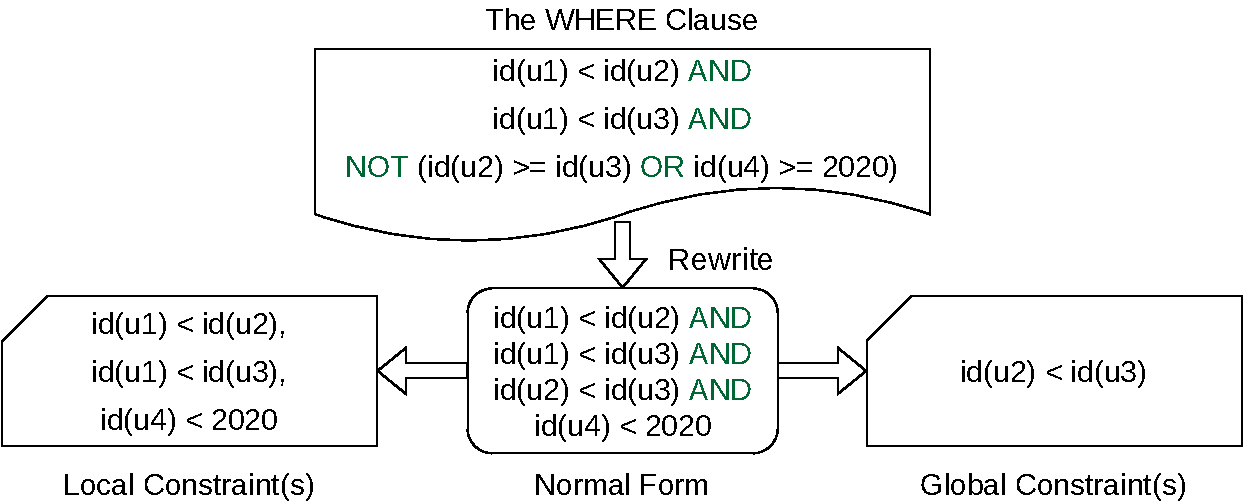
\includegraphics[width=.45\textwidth]{img/constraints.pdf}
  \caption{Constraint Analysis.}\label{img:constraints}
\end{figure}

To address this problem, as shown in Figure~\ref{img:constraints},
we dive into the syntax tree of the graph matching query and decompose the searching condition into smaller parts which require only what we could got during the graph matching phase.
Specifically, we decompose the searching condition into three parts: \emph{vertex constraints}, \emph{edge constraints} and \emph{global constraint}.
A vertex constraint is a function $\psi(u)$ mapping vertex $u$ to Boolean values,
and an edge constraint sets a constraint on edge $(u_1, u_2)$ by a function $\psi(u_1, u_2)$.
For example, in Figure~\ref{img:pattern} ``\mintinline{cypher}{id(u4) < 2020}'' sets a vertex constraint on $u_4$,
``\mintinline{cypher}{id(u1) < id(u2)}'' and ``\mintinline{cypher}{id(u1) < id(u3)}'' are edge constraints,
while ``\mintinline{cypher}{id(u2) < id(u3)}'' is not because there is no edge between $u_2$ and $u_3$.
\textbf{The \emph{vertex constraints} and \emph{edge constraints} are \emph{local constraints} that only require local information that can be obtained during the graph matching phase.
So they could then be pushed down to the data graph scanning phase to short-circuit useless matching results.}
A global constraint $\psi(u_1, u_2, \dots)$ sets a constraint on a series of vertices $u_1, u_2, \dots$,
the information is insufficient during the data graph scanning phase,
however, it still contains many useful information that can be used during the join phase,
and we will discuss it later in Section~\ref{sec:join_on_compressed_data}.

\begin{algorithm}[ht]
  \caption{Constraint Rewriting}\label{alg:rewrite}
  \SetKwFunction{ConstraintRewrite}{\textsc{ConstraintRewrite}}
  \SetKwFunction{Simplify}{\textsc{Simplify}}
  \Input{$expr$: the abstract syntax tree of the WHERE clause}
  \Output{A set of simplified constraints connected by the AND ($\land$) operator}
  \Fn{\ConstraintRewrite{$expr$}}{
    \Match{$expr$}{
      \Case{$\lnot \lnot e$}{\Return{\ConstraintRewrite{$e$}}}
      \Case{$\lnot (e_1 \lor e_2)$}{
        \Return{\ConstraintRewrite{$\lnot e_1$} $\cup$ \ConstraintRewrite{$\lnot e_2$}}
      }
      \Case{$e_1 \land e_2$}{\Return{\ConstraintRewrite{$e_1$} $\cup$ \ConstraintRewrite{$e_2$}}}
      \Case{$e$}{\Return{$\{$ \Simplify{$e$} $\}$}}
    }
  }
\end{algorithm}

Logically, the AND ($\land$) operator create a new constraint $\psi = \psi_1 \land \psi_2$ by combining two constraints $\psi_1$ and $\psi_2$,
where $\psi_1$ and $\psi_2$ can be used to check the matching results independently because there is no side effects in constraints,
so we could safely split $\psi$ into $\psi_1$ and $\psi_2$.
\textbf{Because local constraints are the earliest constraint filters, we should extract as much as possible.}
In order to make the constraint filters more efficient and extract more local constraints:
Firstly, we optimize the AST by classic methods such as compile-time calculation,
handle special cases such as ``\mintinline{cypher}{WHERE false}''.
Then, we apply Algorithm~\ref{alg:rewrite} to analyze the syntax tree and rewrite it into \emph{normal form},
where a normal form is a list of simplified constraints connected by the AND operator.
In fact, the constraints are mostly specified by binary operators such as ``$\le$'', ``$\ne$'',
hence many constraints are naturally local constraints.
And the De Morgan's law enables us to convert the OR ($\lor$) operator into AND ($\land$):
\begin{equation}
  \lnot (\psi_1 \lor \psi_2) = \lnot \psi_1 \land \lnot \psi_2
\end{equation}
So Algorithm~\ref{alg:rewrite} will always keep the semantics of the original user provided constraint.
For example, the third predicate of the AND operator in Figure~\ref{img:cypher_query} would be rewritten to
\begin{minted}[fontsize=\scriptsize]{cypher}
  id(u2) < id(u3) AND id(u4) < 2020
\end{minted}
by applying De Morgan's law.
And the WHERE clause of Figure~\ref{img:cypher_query} would be rewritten to the normal form:
\begin{minted}[fontsize=\scriptsize]{lisp}
  WHERE id(u1) < id(u2) AND id(u1) < id(u3)
  AND id(u2) < id(u3) AND id(u4) < 2020
\end{minted}

\begin{algorithm}[ht]
  \caption{Constraint Pushdown}\label{alg:push_down}
  \SetKwFunction{ConstraintPushdown}{\textsc{ConstraintPushdown}}
  \SetKwFunction{AddVertexConstraint}{\textsc{AddVertexConstraint}}
  \SetKwFunction{AddEdgeConstraint}{\textsc{AddEdgeConstraint}}
  \SetKwFunction{Edges}{\textsc{Edges}}
  \Input{The normal form of constraints $exprs$ and the user described pattern graph $p$}
  \Output{The vertex constraints and edge constraints are pushed down to $p$ and the global constraints will be returned}
  \Fn{\ConstraintPushdown{$exprs$, $p$}}{
    $globals \leftarrow [\,]$\;
    \ForEach{$expr \in exprs$}{
      \Match{$expr$}{
        \Case{$\psi(u)$}{\AddVertexConstraint{$p$, $\psi(u)$}}
        \Case{$\psi(u_1, u_2)$}{
          \If{$(u_1, u_2) \in$ \Edges{$p$}}{\AddEdgeConstraint{$p$, $u_1$, $u_2$, $\psi(u_1, u_2)$}}
        }
        \Case{$e$}{$globals \leftarrow globals \cup \{e\}$\;}
      }
    }
    \Return{$globals$}
  }
\end{algorithm}

The normal form is then used to extract useful information to be pushed down to the pattern graph as in Algorithm~\ref{alg:push_down}.
For each constraint in the normal form, we check if it is local constraint and then push it down to the corresponding vertex or edge.
For example, we would obtain the pattern graph in Figure~\ref{img:pattern_constraint} after doing constraint analysis for the query in Figure~\ref{img:cypher_query}.
After that, We could then decompose it into stars (Section~\ref{sec:star_decomposition}).
Our framework contains a JIT compiler that is able to emit callable closures based on the AST,
and the local constraints can then be used to serve as early filters in the data graph scanning process to short-circuit unnecessary matchings as soon as possible (Section~\ref{sec:data_graph_scanning}).
\begin{figure}[ht]
  \centering
  \resizebox{.7\columnwidth}{!}{
    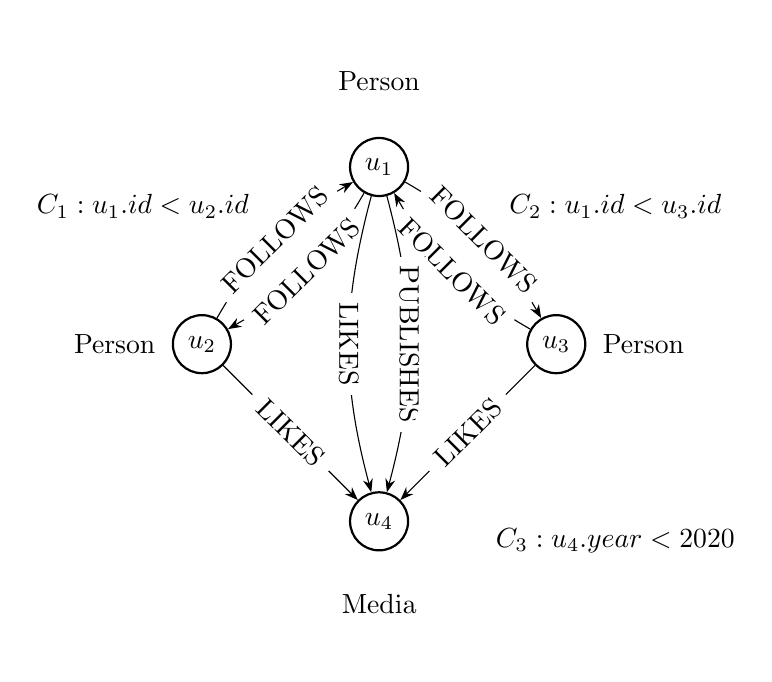
\begin{tikzpicture}
      \begin{scope}
        \node (C1) at (-3, 1.75) {$C_1: u_1.id < u_2.id$};
        \node (c2) at (3, 1.75) {$C_2: u_1.id < u_3.id$};
        \node (c4) at (3, -2.5) {$C_3: u_4.year < 2020$};
      \end{scope}
      \begin{scope}[every node/.style={circle,thick,draw}]
        \node[label={[label distance=0.6]90:Person}] (1) at (0, 2.25) {$u_1$};
        \node[label={[label distance=1]180:Person}] (2) at (-2.25, 0) {$u_2$};
        \node[label={[label distance=1]0:Person}] (3) at (2.25, 0) {$u_3$};
        \node[label={[label distance=0.6]270:Media}] (4) at (0, -2.25) {$u_4$};
      \end{scope}
      \begin{scope}[>={Stealth[black]},
          every node/.style={fill=white,circle},
          every edge/.style={draw=black}]
        \path [->] (1) edge[bend left=15] node[rectangle,rotate=45] {FOLLOWS} (2);
        \path [->] (2) edge[bend left=15] node[rectangle,rotate=45] {FOLLOWS} (1);
        \path [->] (1) edge[bend left=15] node[rectangle,rotate=-45] {FOLLOWS} (3);
        \path [->] (3) edge[bend left=15] node[rectangle,rotate=-45] {FOLLOWS} (1);
        \path [->] (1) edge[bend left=15] node[rectangle,rotate=-90] {PUBLISHES} (4);
        \path [->] (1) edge[bend right=15] node[rectangle,rotate=-90] {LIKES} (4);
        \path [->] (2) edge node[rotate=-45] {LIKES} (4);
        \path [->] (3) edge node[rotate=45] {LIKES} (4);
      \end{scope}
    \end{tikzpicture}
  }
  \caption{The pattern graph with local constraints pushed down.}\label{img:pattern_constraint}
\end{figure}
\subsection{Star Decomposition}\label{sec:star_decomposition}
\textbf{To design a join based graph matching algorithm, the first thing is to decide what is the basic join unit.}
The simplest join unit is edge, however, it will result in huge amount of useless intermediate results if we use edge as basic unit.
Some authors may adopt more complex structure such as frequent subgraphs as their basic unit,
however, super-linear indices are inevitable for these algorithms~\cite{DBLP:journals/pvldb/SunWWSL12},
and this problem would be more severe for out-of-core environment.
Based on these observations, \textbf{we make a balance by adopting star as our basic matching unit},
where a star $S_k$ is a complete bipartite graph $K_{1,k}$ with one root and $k$ leaves.
For one thing, stars can be matched sequentially without complex indices in a out-of-core environment,
which we will discuss more details in the next section.
And for another, stars can hold enough information, both structural information of the pattern graph and the additional searching constraints provided by user's WHERE clause, to reduce the size of intermediate results.
In this section, we will show how to keep these information as much as possible by decompose the pattern graph into stars properly.

\begin{algorithm}[ht]
  \caption{Star Decomposition}\label{alg:decompose_stars}
  \SetKwFunction{DecomposeStars}{\textsc{DecomposeStars}}
  \SetKwFunction{Peek}{\textsc{Peek}}
  \SetKwFunction{Star}{\textsc{Star}}
  \SetKwFunction{RemoveVertex}{\textsc{RemoveVertex}}
  \Input{The pattern graph $p$ with vertex/edge constraints pushed down}
  \Output{A sequence of stars with a specific order}
  \Fn{\DecomposeStars{$p$}}{
    $results \leftarrow [\,]$\;
    $p' \leftarrow p$\;
    $candidates \leftarrow \{u | \max_{u \in \text{Vertices}(p)}f(u)\}$\;
    \While{$candidates \neq \emptyset$}{
      $root \leftarrow$ \Peek{$candidates$}\;
      $candidates \leftarrow candidates \setminus \{ root \}$\;
      $candidates \leftarrow candidates \cup \{ leaf \mid leaf \text{ is adjacent to } root \text{ in } p'\}$\;
      \RemoveVertex{$p'$, $root$}\;
      $candidates \leftarrow candidates \setminus \{ u \mid u \in p' \land \deg{u} = 0 \}$\;
      $results \leftarrow results \cup \{$ \Star{$p$, $root$} $\}$\;
    }
    \Return{$results$}
  }
\end{algorithm}

As many authors have stated before,
\textbf{the matching order has a significant impact on the performance of a graph matching query}~\cite{DBLP:journals/pvldb/SunWWSL12,DBLP:conf/sigmod/HanLL13,DBLP:journals/pvldb/LaiQLC15}.
In our framework, matching order is determined by the stars' root order.
We conclude that the root order affects the overall performance in two aspects:
First, different matching orders result in different join operations which have different performance.
Second, the size of the star matching result is determined by the root selection.
Hence, we provide two rules respectively to guide the star decomposition algorithm (Algorithm~\ref{alg:decompose_stars}):
\begin{itemize}[noitemsep]
\item The root should be selected in the leaves of the previous star except for the first star.
\item We prefer to select the vertex $u$ such that $f(u)$ is the maximum among the candidates,
  where $f(u) = \frac{\deg \times nc}{freq}$ is a heuristic function on the degree $\deg$ of $u$,
  number of constraints $nc$ and the frequency $freq$ of vertices with the same label of $u$ in the data graph.
\end{itemize}

The first rule indicates that the roots would form a connected vertex cover of the original pattern graph step by step.
\textbf{By doing so, the join operation will always occurred between two adjacent stars},
and we could use a simple index to boost the join operation (Section~\ref{sec:join_on_compressed_data}).
In contrast, for example, if the two stars are totally separated without any common vertices,
then the join result of these stars would be the Cartesian product of respective star matching results,
where most of the rows in the Cartesian product would be invalid.
The Second rule considers both the information of the pattern graph and the distribution of data graph.
We prefer to select root that contains more structural constraints ($\deg$) and user provided constraints ($nc$),
and prefer root with a low label frequency in the data graph.
\textbf{By doing so the matching result of the star could be as small as possible which reduces the I/O cost and alleviates the burden of the later join operation.}

Previous work STwig~\cite{DBLP:journals/pvldb/SunWWSL12} and TwinTwig~\cite{DBLP:journals/pvldb/LaiQLC15} also use stars as their basic matching units.
However, unlike these previous work which are designed for simple graphs, our stars fully support the real-world property graph model, and most importantly, we will show that the star decomposition algorithm of previous work has a lot of room to be optimized.

\textbf{Both STwig and TwinTwig are designed for undirected simple graph,
which has a limited expressiveness and is not suitable for many real-world applications.}
In contrast, we adopt the property graph model which is widely used in industrial graph databases.
Figure~\ref{img:stars} shows the decomposition results of the patter graph in Figure~\ref{img:pattern},
both vertices and edges are labeled and multiple edges may exist between a leaf and the root vertex.
The vertex constraint $C_4$ and edge constraints $C_1$, $C_2$ are also shown in the graph.

\begin{figure}[ht]
  \centering
  \resizebox{.6\columnwidth}{!}{
    \begin{tikzpicture}
      \begin{scope}[every node/.style={circle,thick,draw}]
        \node[label={[label distance=0.6]90:Person}] (1) at (0, 2.25) {$u_1$};
        \node[label={[label distance=1]180:Person}] (2) at (-2.25, 0) {$u_2$};
        \node[label={[label distance=1]0:Person}] (3) at (2.25, 0) {$u_3$};
        \node[label={[label distance=0.6]270:Media}] (4) at (0, -2.25) {$u_4$};
      \end{scope}
      \begin{scope}[>={Stealth[black]},
          every node/.style={fill=white,circle},
          every edge/.style={draw=black}]
        \path (1) edge (2);
        \path (1) edge (3);
        \path (1) edge (4);
      \end{scope}
    \end{tikzpicture}
  }
  \resizebox{.6\columnwidth}{!}{
    \begin{tikzpicture}
      \begin{scope}[every node/.style={circle,thick,draw}]
        \node[label={[label distance=1]180:Person}] (2) at (-2.25, 0) {$u_2$};
        \node[label={[label distance=1]0:Person}] (3) at (2.25, 0) {$u_3$};
        \node[label={[label distance=0.6]270:Media}] (4) at (0, -2.25) {$u_4$};
      \end{scope}
      \begin{scope}[>={Stealth[black]},
          every node/.style={fill=white,circle},
          every edge/.style={draw=black}]
        \path (2) edge (4);
        \path (3) edge (4);
      \end{scope}
    \end{tikzpicture}
  }
  \caption{The stars generated by previous algorithms.}\label{img:stars_old}
\end{figure}

\textbf{Apart from the graph model differences, we found that existing query decomposition algorithms still have a a lot of room to be improved.}
As we discussed before, the result of the data graph scanning process should be as small as possible to avoid unnecessary I/O cost.
The leaves of a star graph can be viewed as a bunch of constraints on the root vertex,
which help to eliminate useless mappings of the root.
That is to say: \emph{more leaves, more better}.
However, \textbf{previous work ignore the benefits of leaves and leave a lot of room to be optimized}.
Compared to the decomposition result of previous work in Figure~\ref{img:stars},
our algorithm always keeps all the leaves in the pattern graph,
while, the stars of previous work drop many useful leaves.
In some cases, e.g., triangle graph, they even generate stars with only two vertices which reduce to edge decomposition.
Apparently, an edge will result in much more unnecessary matchings than a star.

The key of the optimization of our algorithm is the use of $p'$:
We first copy the pattern graph $p$ and obtain $p'$.
Then we run the vertex cover finding algorithm on $p'$,
vertices are removed one by one in $p'$ while $p$ is always unchanged.
Finally, we use the original $p$ to induce stars.
So the resulting stars will always hold as much leaves as possible,
which improves the performance of data graph scanning significantly.
Experiments show that this simple optimization can reduce the size of matching results to \@???\% of previous work.
\subsection{Data Graph Scanning}\label{sec:data_graph_scanning}
Now, we are ready to elaborate how we match stars efficiently in an out-of-core environment.
First, we will propose our stars matching algorithm by introducing two iterators.
And then we'll show how to implement the two iterators by designing a novel disk format to store the data format,
such that the star matching process is I/O efficient, where \textbf{the huge data graph will be read sequentially without random access, and read at most once}.
\subsection*{Stars Matching}
Random disk access problem is always a challenging problem for out-of-core systems,
especially for the out-of-core graph matching problem where graphs are notorious for their poor locality.
However, in this section, we will show that we could avoid random disk accesses by matching stars using two simple iterators.
Furthermore, our techniques ensure that we would only read the necessary part from the huge data graph file,
and these necessary parts would be only read sequentially once.
That is to say, \textbf{we could match all the stars by scanning only the necessary part of the data graph file sequentially once}.

Consider the first star $star_1$ in Figure~\ref{img:stars}, the root vertex is $u_1$ with the label ``Person'',
and it has three leaves $u_2$, $u_3$ and $u_4$.
To match such a star in a data graph, we should find a star whose root also contains the label ``Person''
and it has at least 3 neighbors that could match $u_2$, $u_3$ and $u_4$ respectively.
Then it is straightforward to obtain an naive method to match $star_1$ in a data graph $d$:
Iterate through \textsc{VertexIter}$(d, Person)$ and check every neighbors of these vertices whether they could match $u_2$, $u_3$ and $u_4$, where \textsc{VertexIter}$(d, l)$ travels through all the vertices with the label $l$ in the data graph $d$.
For example, in Figure~\ref{img:data}, $d[v_1]$, the induced graph of $d$ on $v_1$, is such a star that could match $star_1$.

However, this naive star matching method has a great drawback for vertices with a high degree.
Consider the second star $star_2$ in Figure~\ref{img:stars}, the root vertex is $u_4$ with the label ``Media''.
And we suppose that in Figure~\ref{img:data}, $v_4$ is such a popular media that millions or even billions of persons have left their likes.
The naive method have to visit all the neighbors of $v_4$ but most of them are useless because there is no vertex with label ``Comment'' in $star_2$.
To solve this problem, we introduce the second iterator \textsc{NeighborIter}$(v, l)$,
which visits the neighbors with the label $l$ of a given data vertex $v$.
By iterating through \textsc{NeighborIter}$(v_4, Person)$, we could skip useless neighbors and only load the necessary ones.

\begin{definition}[VertexIter and NeighborIter]
  In a data graph $d$, given a vertex label $l$, \textsc{VertexIter}$(d, l)$ is a iterator that would visit all the vertices with the label $l$ in $d$ sequentially.
  Given a data vertex $v$ and a vertex label $l$, \textsc{NeighborIter}$(v, l)$ is a iterator that would iterate through the neighbors with label $l$ of $v$ sequentially.
\end{definition}

Now we will answer the question: How to match the neighbors with the help of \textsc{NeighborIter}?
Consider $star_1$ in Figure~\ref{img:stars}, it is easy to find the symmetry in this star.
We say that $u_2$ and $u_3$ are equivalent because they have the same vertex label,
their connections to the root are the same, and the edge constraints $C_1$ and $C_2$ are also equivalent
(Remember that an edge constraint is a function, that in this case $u_2$ and $u_3$ are just free variables).
For simplicity, we introduce the definition \textsc{NeighborInfo} as follows:
\begin{definition}[NeighborInfo]
  A \textsc{NeighborInfo} of a neighbor vertex $n$ is a structure that stores:
  \begin{enumerate}[noitemsep]
  \item the label of the neighbor $n$,
  \item the vertex constraint of the neighbor $n$,
  \item the edges between the root vertex $v$ and the neighbor $n$
    (the direction of the edges may be $v \rightarrow n$, $v \leftarrow n$ or $v \text{---} n$ because a user could ignore the direction of some edges in the pattern graph),
  \item and the edge constraints of the edges.
  \end{enumerate}
\end{definition}
In a star graph, \textbf{the leaves with the same \textsc{NeighborInfo} form a equivalence class,
and there is no need to blindly permute all possible mappings for the vertices in the same \textsc{NeighborInfo} equivalence class}.
Suppose that there are $m$ leaves with the same \textsc{NeighborInfo} in a star, for each leaf there are $n$ vertices that could be matched in the data graph.
We have to use $m!n$ rows to store the matching result if we blindly permute the mappings for the leaves.
In contrast, only $n$ rows are required if we match group these leaves together which reduces I/O cost dramatically.
\textbf{So instead of matching each neighbors directly, we group the leaves of the star pattern graph by their \textsc{NeighborInfo} during the static analyzing phase, and then use the \textsc{NeighborInfo} to match equivalent vertices at the same time.}
For each neighbor in the \textsc{NeighborIter}, we check whether it would be matched by,
firstly, checking the local constraints of the neighbor,
and then checking the edges between the root and the neighbor.

\begin{algorithm}[ht]
  \caption{Stars Matching}\label{alg:match_stars}
  \SetKwFunction{MatchStars}{\textsc{MatchStars}}
  \SetKwFunction{VertexIter}{\textsc{VertexIter}}
  \SetKwFunction{NeighborIter}{\textsc{NeighborIter}}
  \SetKwFunction{InitializeResults}{\textsc{InitializeResults}}
  \SetKwFunction{AppendResult}{\textsc{AppendResult}}
  \SetKwFunction{FinalizeResults}{\textsc{FinalizeResults}}
  \SetKwFunction{VertexConstraint}{\textsc{VertexConstraint}}
  \SetKwFunction{DegreeConstraint}{\textsc{DegreeConstraint}}
  \SetKwFunction{MatchNeighbor}{\textsc{MatchNeighbor}}
  \SetKwFunction{MatchNeighborInfo}{\textsc{MatchNeighborInfo}}
  \SetKwFunction{Flatten}{\textsc{Flatten}}
  \SetKwFunction{NeighborInfos}{\textsc{NeighborInfos}}
  \Input{The data graph $d$ and a list of $stars$ with the same root label}
  \Output{A list of compressed star matching $results$ corresponding to the $stars$}
  \Fn{\MatchStars{$d$, $stars$}}{
    $results \leftarrow$ \InitializeResults{$stars$}\;
    \ForEach{$v \in$\VertexIter{$d$, $stars[0].root.vlabel$}}{
      $candidates \leftarrow \{ star | star.root$.\VertexConstraint{$v$} $\land star.root$.\DegreeConstraint{$v$} $\}$\;
      $nlabel\_stars \leftarrow $ groups the $candidates$ by leaves' label\;
      \ForEach{$(nlabel, stars) \in nlabel\_stars$}{
        \ForEach{$n \in$\NeighborIter{$v$, $nlabel$}}{
          \MatchNeighbor{$v$, $n$, stars, results}\;
        }
      }
    }
    \FinalizeResults{$results$}\;
    \Return{$results$}\;
  }

  \Fn{\MatchNeighbor{$v$, $n$, $stars$, $results$}}{
    \ForEach{$star \in stars$}{
      \ForEach{$info \in star$.\NeighborInfos{$n.vlabel$}}{
        \If{\MatchNeighborInfo{$v$, $n$, $info$}}{
          \AppendResult{$results[star]$, $n$}\;
        }
      }
    }
  }
\end{algorithm}

By far, there is only one challenge left: How to scan the huge data graph file only once?
The size of the data graph file is proportional to the number of edges in the data graph.
Existing in-memory algorithms would visit the vertices back and forth to explore the data graph,
naively adopt these algorithms to the out-of-core environment would result in numerous swap in/outs,
which is very time consuming and I/O inefficient.
An algorithm that only scan the data graph file sequentially once is desirable,
and we propose a positive answer by providing Algorithm~\ref{alg:match_stars}.
Consider the stars in Figure~\ref{img:stars}, there are two stars that the labels of the roots are different.
\textsc{VertexIter}$(d, Person)$ and \textsc{VertexIter}$(d, Media)$ would be used to visit the vertices in the data graph $d$.
If the data vertices with the same label are stored together in disk,
then the \textsc{VertexIter} could load only the necessary part from disk and visit the vertices sequentially.
Generally speaking, if there are $n$ stars generate by Algorithm~\ref{alg:decompose_stars},
and the size of the labels of the roots is $m$, we have $m \le n$ since multiple stars may have the same label of root.
\textbf{Then we could use $m$ different \textsc{VertexIter} to scan the data graph file by grouping same-label-of-root stars together,
and every iterator would only load a distinct part of the data graph sequentially}
(There is a special case that some stars may isomorphic,
and there is no need to do duplicate star matching, Section~\ref{sec:equivalence_classes} would discuss it in detail).
\textbf{Macroscopically, only the necessary part of the data graph would be loaded to match a pattern graph,
and these parts would be read sequentially only once with the help of \textsc{VertexIter} and \textsc{NeighborIter}.}
\subsection*{Data Graph Disk Format}
To implement the two iterators efficiently, we design a compact disk format to store the data graph (Figure~\ref{img:data_disk_format}).
The disk format is a little bit like to the conventional adjacency list format,
that is, we store a vertex and it's neighbors together.

Specifically, in order to implement the \textsc{VertexIter} efficiently,
\textbf{we should locate data vertices efficiently given a vertex label and visit these vertices without random disk access}.
So \textbf{we store vertices with same vertex label adjacently, and adopt a simple label-to-\textsc{VertexIter} index to boost the searching}.
The \mintinline{text}{num_bytes} field would be used to calculate the position of the next data vertex,
such that the \textsc{VertexIter} can visit the data vertices on disk sequentially to reduce I/O cost.
Apart from that, we also store in-degree and out-degree which can be used as early filters during the star matching process.

For the \textsc{NeighborIter}, there is one thing to notice that we adopt the property graph model,
all edges are directed and multi-edges may exist between a pair of vertices.
To store these information, a naive method is to store in-edges and out-edges for each data vertex.
However, this naive method will be very inefficient when matching property graphs.
Consider the pattern graph in Figure~\ref{img:pattern},
suppose that in a data graph $v_1$ matches $u_1$ and we want to check whether $v_2$, a neighbor of $v_1$, matches $u_2$,
then we have to scan all the in-edges to find if there is an edge from $v_2$ to $v_1$ with label ``FOLLOWS'',
and all the out-edges to check if there is an edge from $v_1$ to $v_2$ with the same label.
Real-world graphs usually have a high skewness, for example, a celebrity in a social network may have millions of followers.
\textbf{These ``celebrities'' will become bottleneck if we adopt the naive method to scan all the adjacent edges.}
To solve this problem, we propose a novel schema to store the neighbors,
\textbf{all the edges connected to a neighbor are stored together with the neighbor,
so the neighbor can be checked in place without scanning all the in-edges/out-edges of the root vertex}.
And we also use a simple label-to-\textsc{NeighborIter} index to boost the searching of neighbors given the label of neighbor.
The position of the next neighbor could be calulated by the \mintinline{text}{num_n_to_v} and \mintinline{text}{num_v_to_n} fields.
And we could use \textsc{NeighborIter} to travel through the neighbors sequentially without random disk access.

\begin{figure}[ht]
  \centering
  \begin{minted}[fontsize=\tiny]{text}
+-----------------------------------------+
|             num_vlabels: k              |
+-----------------------------------------+
+-------------+-------------+-------------+
|   vlabel    |     pos     |     len     |<-+
+-------------+-------------+-------------+  |
|   vlabel    |     pos     |     len     |  |
+-------------+-------------+-------------+  |- k rows
                    ...                      |
+-------------+-------------+-------------+  |
|   vlabel    |     pos     |     len     |<-+
+-------------+-------------+-------------+
+--------------------+--------------------+
|     num_bytes      |         v          |<-----------------------------+
+--------------------+--------------------+                              |
|      in_deg        |      out_deg       |                              |
+--------------------+--------------------+                              |
|               num_vlabels               |                              |
+-----------------------------------------+                              |
+-------------+-------------+-------------+                              |
|   vlabel    |     pos     |     len     |<-+                           |
+-------------+-------------+-------------+  |                           |
|   vlabel    |     pos     |     len     |  |                           |
+-------------+-------------+-------------+  |- num_vlabels rows         |
                    ...                      |                           |
+-------------+-------------+-------------+  |                           |
|   vlabel    |     pos     |     len     |<-+                           |
+-------------+-------------+-------------+                              |     One
+-----------------------------------------+                              |- VertexNode
|                    n                    |                              |
+--------------------+--------------------+                              |
|    num_n_to_v      |    num_v_to n      |                              |
+--------------------+--------------------+                              |
+-----------------------------------------+                              |
|                 elabel                  |<-+                           |
+-----------------------------------------+  |                           |
|                 elabel                  |  |  num_n_to_v + num_v_to_n  |
+-----------------------------------------+  |-           rows           |
                    ...                      |                           |
+-----------------------------------------+  |                           |
|                 elabel                  |<-+                           |
+-----------------------------------------+                              |
                    ...                    <-----------------------------+

  \end{minted}
  \caption{Data graph disk format. (TODO\@: Update this figure.)}\label{img:data_disk_format}
\end{figure}

The vertices are sorted by their ID in the data graph, which is very helpful for the join operation (Section~\ref{sec:join_on_compressed_data}).
Given a series of vertices and a series of edges with arbitrary order,
the data graph file could be generated in sorting time.
And for simplicity, we ignore the key-value properties of a property graph and focus on the labels.
In fact, these properties can be added to our disk format by simply add the corresponding fields.
And the simplicity of the \textsc{VertexIter} and \textsc{NeighborIter} also makes it possible to implement them on other platform, e.g., industry-tested relational database, which we will study in future work to make dynamic property graph transactions and analysis easier.

\section{Vertex-Centric Storage for Property Graph}\label{sec:storage}
%The random access problem is a well known hard problem for out-of-core systems, especially for the graph related problem, which is notorious for its poor locality~\cite{DBLP:conf/osdi/KyrolaBG12}.

Many graph computing frameworks store graphs on disk using the double list method:
storing the in-edges and out-edges \textbf{separately} for each vertex,
via the compressed sparse column (CSC) and the compressed sparse row (CSR) format~\cite{DBLP:conf/sc/PearceGA10}.
However, this separation incurs excessive random access on real-world property graph because we need to get the information for in/out edges during pattern matching.

Instead, SeqStar stores the graph data in a vertex-centric way which stores all the information related to one vertex \textbf{together}.
With small indexes on disks, pattern matching can quickly get the correct address of relevant data on disk during pattern matching. Because all the related information is stored together, SeqStar can make sure that all disk reads are sequential.

Moreover, by using the property graph matching engine that will be discussed in the next section,
the huge data graph will be read at most once.
\subsection{Scan the Data Graph Sequentially}
%The property graph matching problem requires the complete connection information between vertices,
%however, the conventional double list storage method break up the completeness and results in random disk accesses.

Consider the example in Figure~\ref{img:running_example}.
If two vertices in the data graph, say $v_i$ and $v_j$, are supposed to match $u_1$ and $u_2$,
we must be sure that $v_i$ and $v_j$ follows each other at the same time.
This kind of neighbor checking is the most essentially building block of a property graph matching engine.

In the data graph, vertex $1$ has $4$ in-edges and $7$ out-edges.
Suppose that they are stored separately in the traditional way.
In order to determine whether vertex $1$ could match $u_1$,
one has to scan the in-edges (or equally, the out-edges) of vertex $1$ and then check whether the visited neighbor is in the out-edges (or in-edges) list.
Such a scan and check method would significantly slow down the graph matching process,
because the checking process results in random disk reads.
For real world power-law graphs, where the celebrities or trending topics have a huge amount of followers, this phenomenon greatly exacerbate the random access problem.
%the in/out-edges lists stored on disk have to be swapped in and out frequently during the scan and check process as a result of the random disk access pattern.
%% Multiple edges between $u_1$ and $u_2$ make things even worse.
%And it would be more complicated if there are more than two edges between $u_1$ and $u_2$ in the pattern graph.

On the contrarily, SeqStor's vertex-centric storage keeps the necessary connection information together for graph matching.
Figure~\ref{img:data_example} shows the logical structure for the data graph in Figure~\ref{img:running_example}.
The specific edge information (direction, types) could be obtained by the stored edge labels, i.e., the top labels associate to the out-edges and the bottom labels associate to the in-edges (Figure~\ref{img:data_example}).

\begin{figure}[ht]
  \centering
  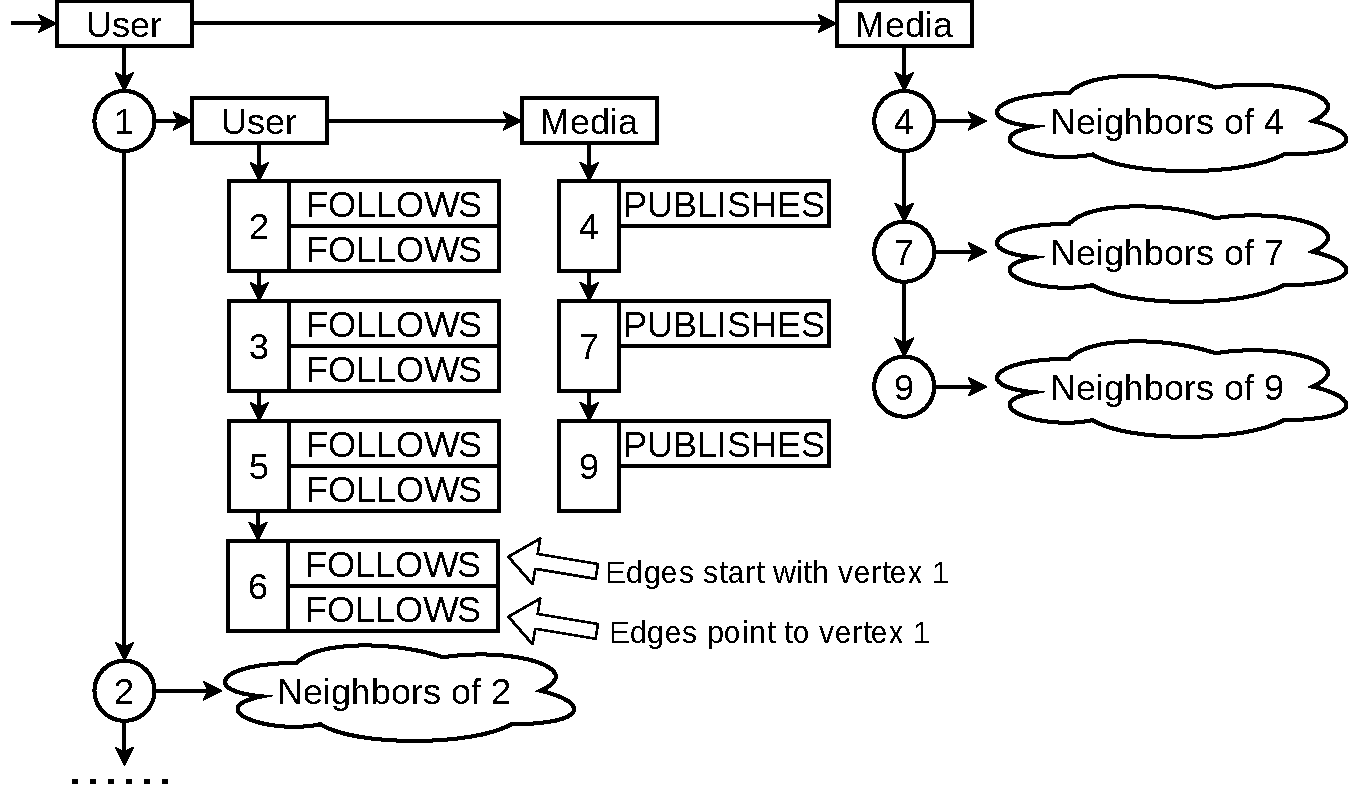
\includegraphics[width=0.5\textwidth]{img/data_example.pdf}
  \caption{Vertex-centric graph data storage.}\label{img:data_example}
\end{figure}

By using the vertex centric graph data storage, the neighborhood checking process can be accomplished efficiently within a sequential disk scan.
For $S_1$ in Figure~\ref{img:running_example},
to check the neighbors of vertex $1$, SeqStar scans the neighbors $2, 3, 5, 6$ and $4, 7, 9$ sequentially.
No random disk access appears during the whole process.
\subsection{Graph Data Indexes}
%Despite of the fact that the size of the whole data graph could be gigantic,we may only care a fraction of the graph by specify the labels in our query for a concrete graph matching problem.
There are two basic operations in a graph matching engine:
(1) Given a data vertex, retrieve its neighbors with a specific label;
(2) Given a vertex label, retrieve the vertices with the label.
%% In the following paragraphs, we'll show how to make the two operations efficiently by adding a few simple but efficient indices to the vertex-centric storage engine,
%% which reduces the searching space and I/O significantly.

Consider the data graph in Figure~\ref{img:running_example}.
One may want to study only the relationships among users.
For vertex $1$ in the figure,
no matter how much social media she has published or viewed we could just ignore all of them in this specific problem.
%% A straightforward idea is to group the neighbor vertices with the same label together when storing the vertices.
%% However, if the neighbor vertices were stored in the traditional in/out-edge double lists method,
%% we have to group them twice and then still face the information insufficient problem as we discussed in the previous subsection.
%% As for our vertex-centric storage method,
For SeqStor's vertex-centric storage method,
the index could be added to the storage engine easily as shown in Figure~\ref{img:data_example}.
These indexes are key-value pairs mapping the vertex labels to the starting/ending position of the neighbors on disk.
Since it is used to locate only the neighbors of a specific vertex, we refer to this kind of index as \emph{local index}.
With the help of local index, we could skip all the useless neighbor vertices and only scan the necessary ones.
%% \begin{figure}[ht]
%%   \centering
%%   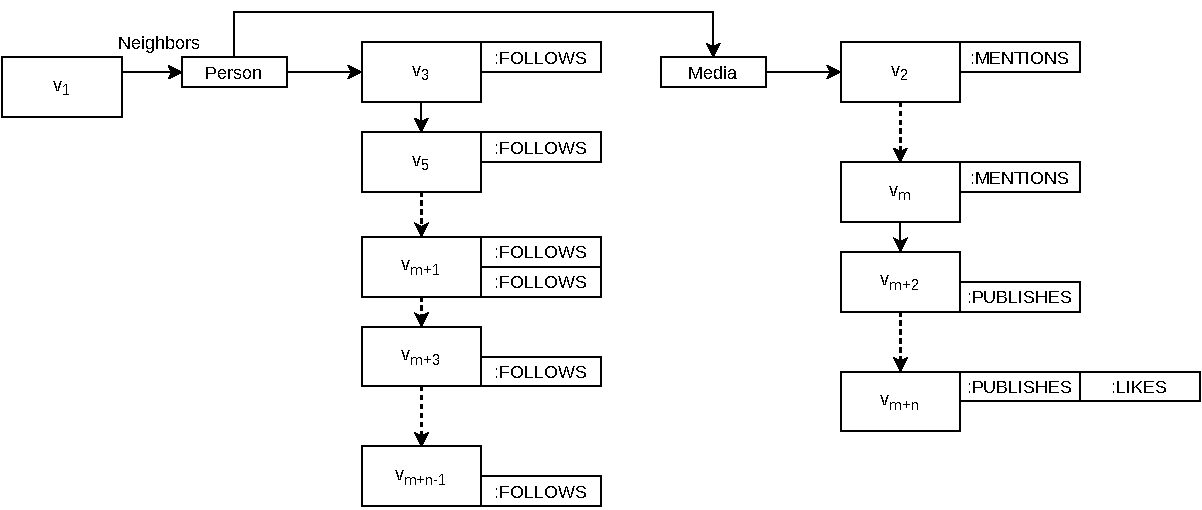
\includegraphics[width=0.48\textwidth]{img/data_neighbors.pdf}
%%   \caption{The vertex-centric storage structure of the celebrity $v_1$ in Figure~\ref{img:celebrity_star}.}\label{img:data_neighbors}
%% \end{figure}

From a higher perspective, in order to solve a property graph matching problem,
one need to firstly select a root vertex in the data graph.
%% regardless of the concrete graph matching algorithm whether it is tree based or join based.
There is no need to scan all the vertices in a billion node data graph if we only care about vertices with the specific labels.
Just like the local index we discussed above, we could add a global index which contains key-value pairs that maps the labels to the corresponding position on disk (Figure~\ref{img:data_example}).

The super-linear index problem of existing work was pointed out by~\cite{DBLP:journals/pvldb/SunWWSL12},
where indexes grow \emph{super-linearly} with respect to the \emph{edges}.
In contrast, indexes of SeqStar grows \emph{linearly} with respect to the \emph{vertices}.
In SeqStar, the length of global index is the length of vertex labels ($l$),
and the size of local indexes is bound to $l \times n$ ($n$ is the length of vertices).
%% In summery, for a property graph matching problem, we could quickly jump to the domain of interest with the help of the global index, and then scan and check only the necessary neighbors with the help of our local index.
%% After jump to the correct position, all the disk reads are sequential.
%% \begin{figure}[ht]
%%   \centering
%%   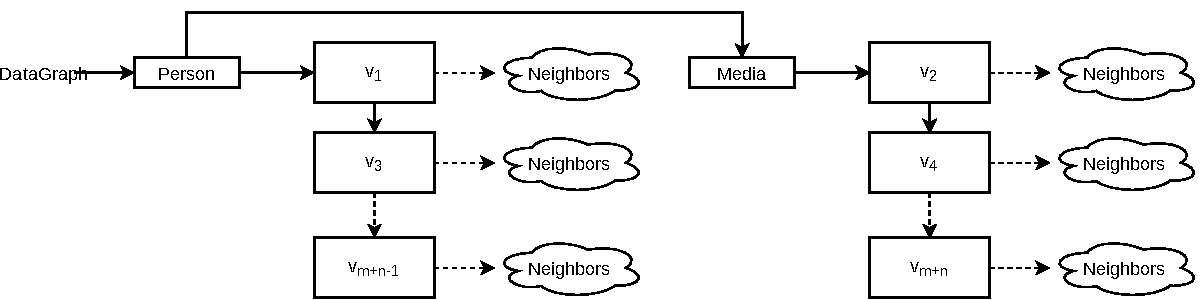
\includegraphics[width=0.48\textwidth]{img/data_vertices.pdf}
%%   \caption{The storage structure overview of the data graph in Figure~\ref{img:celebrity_star}.}\label{img:data_vertices}
%% \end{figure}
\subsection{Remarks on the Implementation of the Storage Method}\label{sec:storage_iterators}
For applications that need to perform the two basic operations (visiting vertices and visiting the neighbors),
we define two iterators as the interface to visit the data graph:
\begin{enumerate}[noitemsep]
\item \textsc{VertexIter}: Given a vertex label, it iterates through the vertices with the specified label ordered by the ID of vertices;
\item \textsc{NeighborIter}: Given a data vertex and a label, it visits the neighbors with the label, the neighbors are also sorted by the IDs.
\end{enumerate}
%% In Section~\ref{sec:match} we'll show that the sorting constraint could boost the matching of property graphs.

These iterators could be implemented efficiently by using SeqStar's vertex-centric storage model.
And we also provide a compact disk format implementing the vertex-centric storage model in Figure~\ref{img:data_graph}.
Vertices are sorted by their IDs, and we store in/out-degrees as early filters when scanning the vertices.
Edge labels are stored as integers here, however, bitmap could also be used for higher performance.
The \textsc{VertexIter} just searches the global index and then visits the disk data sequentially;
The \textsc{NeighborIter} scans the neighbors with the help of the local index.

Note that the vertex-centric storage model is not restricted to this disk format.
In fact, as long as a storage engine could implement the two iterators efficiently,
it could implement the vertex-centric storage model well.
For example, the sorted vertices could be replaced with B-tree to make the insertion/deletion operation easier for dynamic graphs.
%% It is also possible to implement the vertex-centric storage model in memory as buffer cache for existing graph databases to achieve better locality.
Moreover, we are now working on implementing the vertex-centric storage model on top of relational database to embrace the power of the half-century-year-old mature technology.
\begin{figure}[ht]
  \centering
  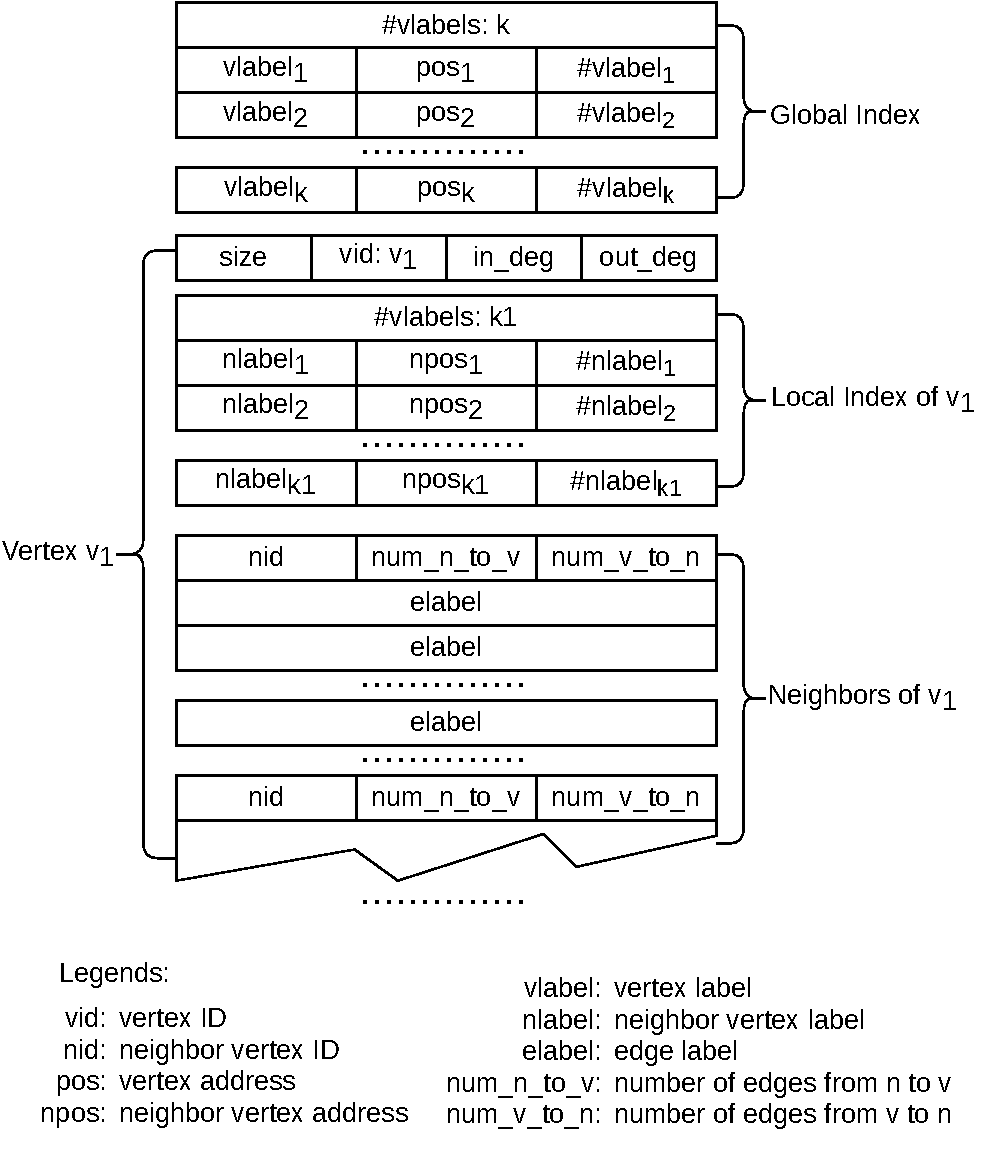
\includegraphics[width=0.48\textwidth]{img/data_graph.pdf}
  \caption{An I/O efficient property graph storage method that can boost the graph matching process.}\label{img:data_graph}
\end{figure}

\section{Evaluation}\label{sec:experiments}
\subsection{Setup}
\subsubsection{Environment}
The experiments were performed on a single machine with two Intel Xeon Processor E5--2699 v4 CPUs, 64 GB of RAM,
and a 800GB SSD\@.
The machine has 22 cores and 44 threads.
Memory caches were dropped before each experiment to force disk loads.
\subsubsection{Datasets and Queries}
We use real-world data graphs~\cite{snapnets} listed in Table~\ref{tab:datasets}.
The datasets come from difference domains of application, and they range in different size.
The vertices and edges in the datasets are labeled randomly as in~\cite{DBLP:journals/pvldb/MhedhbiS19}.

The queries (Figure~\ref{img:queries}) are selected and edited from existing work~\cite{DBLP:conf/cloud/SerafiniMS17,DBLP:journals/pvldb/MhedhbiS19}.
The labels of vertices and edges are tagged randomly,
and they are represented by the color and the style of lines in Figure~\ref{img:queries}.
The queries we choose represent different topologies: trees, chains, and cyclic graphs.
$q_9$ --- $q_{12}$ are queries with multi-edges.
\begin{table}
  \caption{Datasets}\label{tab:datasets}
  \begin{tabular}{lrr}
    \toprule
    Name & $|V|$ & $|E|$ \\
    \midrule
    soc-Epinions (EP) & 76K & 509K \\
    web-Google (GO) & 876K & 5.1M \\
    web-BerkStan (BS) & 685K & 7.6M \\
    soc-LiveJournal (LJ) & 4.8M & 69M \\
    com-Orkut (OK) & 3.1M & 117.2M \\
    \bottomrule
  \end{tabular}
\end{table}

\begin{figure}[ht]
  \centering
  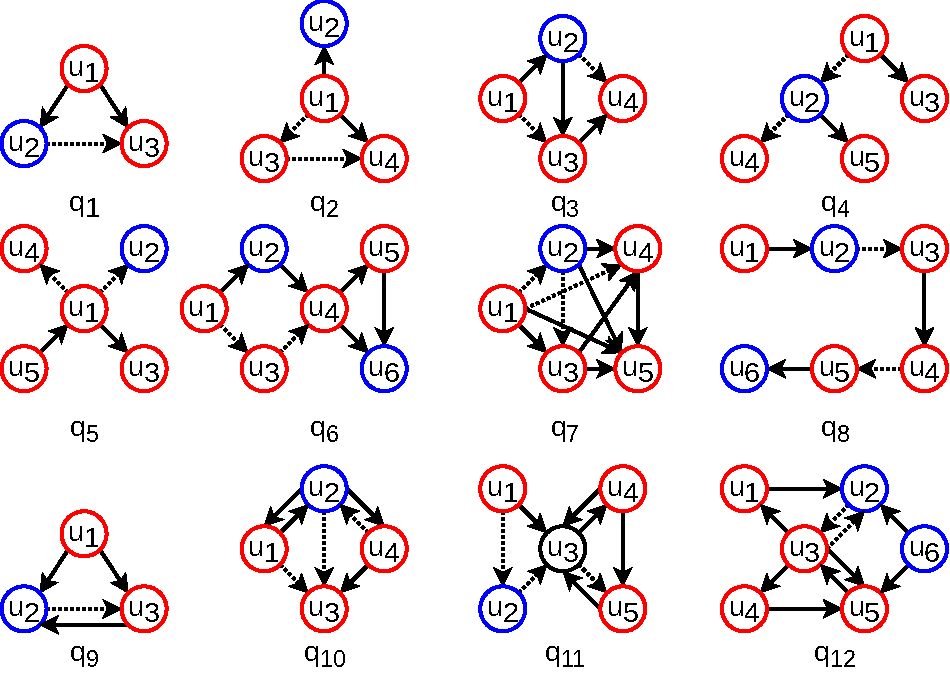
\includegraphics[width=0.5\textwidth]{img/queries.pdf}
  \caption{The queries.}\label{img:queries}
\end{figure}

\subsection{Preprocessing Cost}
We first study the preprocessing cost of SeqStar's vertex-centric storage engine.
The preprocessing incurs a external sort on the original graph data to generate the formatted data graph shown in Figure~\ref{img:data_graph}.
The cost is $\mathcal{O}(n \log n)$ where n is the size of the unsorted graph data.
We use 32-bit integers to store the vertex IDs, and 16-bit integers to store the vertex/edge labels.
As is shown in Figure~\ref{img:exp_preprocessing}, the preprocessing time grows linearly with respect to the size of graph data.
In fact, the preprocessing time of the vertex-centric storage is significantly smaller than the execution time of complex queries.

\begin{figure}[ht]
  \centering
  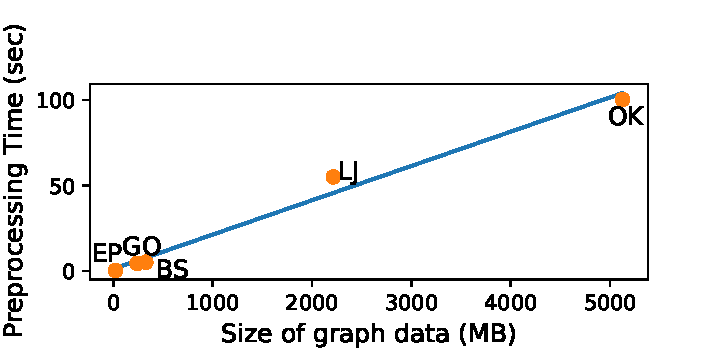
\includegraphics[width=0.4\textwidth]{img/exp_preprocessing.pdf}
  \caption{Preprocessing time of SeqStar.}\label{img:exp_preprocessing}
\end{figure}
\subsection{Comparative Performance}
We compare the overall performance of SeqStar against Graphflow~\cite{DBLP:journals/pvldb/MhedhbiS19} and Neo4j.

Graphflow is the state-of-the-art in-memory subgraph querying system,
and it is the fastest baseline we are aware of.
Graphflow is a JVM based system, and we set the maximum size of the JVM heap to 60GB to let it make full use of main memory.
However Graphflow does not support queries with multi-edges, i.e., $q_9$ --- $q_{12}$,
and it will report fake results for these queries\footnote{Graphflow will report matchings even the data does not contain multi-edges.}.
Therefore we use only $q_1$ --- $q_8$ to compare with Graphflow.
\begin{figure*}[ht]
  \centering
  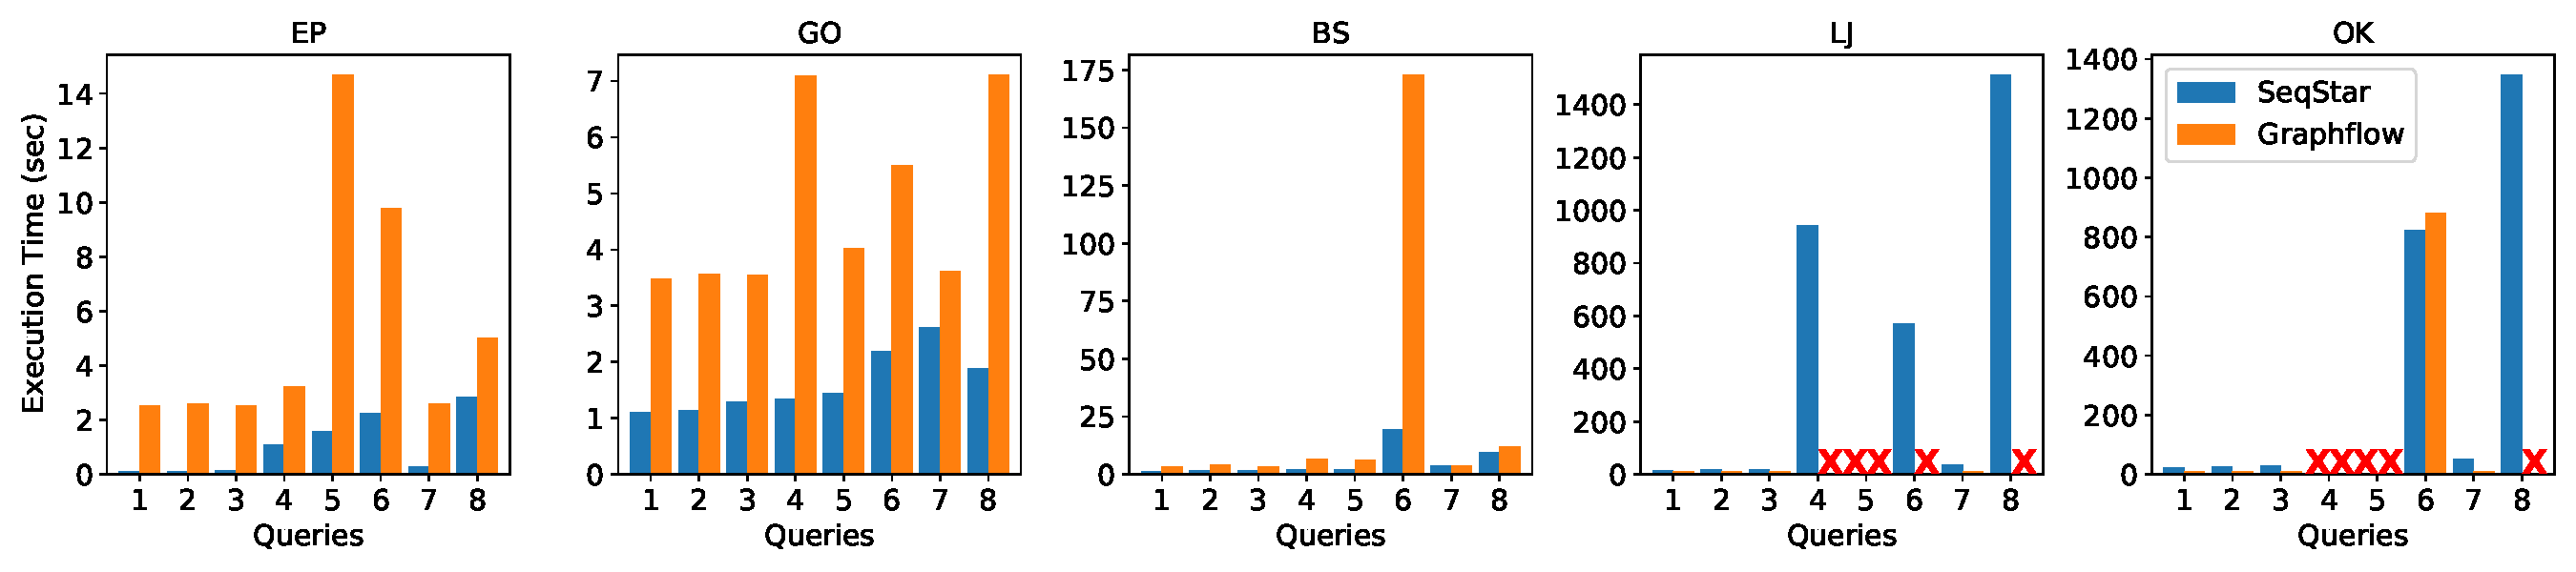
\includegraphics[width=\textwidth]{img/exp_compare.pdf}
  \caption{Execution time.}\label{img:exp_compare}
\end{figure*}

\subsection{Compression Ratio}
\subsection{Performance of Star Decompression}
\subsection{Parallelism of Pipeline Join}

\section{Related Work}
Despite the fact that general property graph matching problem is seldom discussed in previous works,
simple graph matching has been widely studied.
We survey these relevant work in this section.
\subsection*{In-memory Methods}
Most of the early work assumes that the data graph and indices are fit in the main memory of a single machine.
Sparked by Ullmann's backtracking algorithm~\cite{DBLP:journals/jacm/Ullmann76},
many subgraph matching algorithms have been proposed using different searching order, filter rules, and neighborhood indices~\cite{DBLP:journals/pami/CordellaFSV04,DBLP:journals/pvldb/ShangZLY08,DBLP:conf/sigmod/HeS08,DBLP:conf/sigmod/HanLL13,DBLP:journals/pvldb/LeeHKL12}.
These algorithms usually use a DFS-style tree-based graph exploration to search the matchings without materializing intermediate results.
However, these single machine in-memory algorithms are no longer suitable for nowadays billion-node graphs.

To address the scalability problem of single machine in-memory algorithms,
many distributed subgraph matching algorithms have been proposed~\cite{DBLP:journals/pvldb/SunWWSL12,DBLP:conf/sigmod/ShaoCCMYX14,DBLP:journals/pvldb/LaiQLC15,DBLP:journals/pvldb/LaiQLZC16,DBLP:conf/cloud/SerafiniMS17}.
Because the vertices of the data graph are scattered among machines,
these algorithms usually match smaller patterns and get the final result by join operation.
For example, Sun et al.~\cite{DBLP:journals/pvldb/SunWWSL12} introduce a star-like basic matching unit called STwig,
and implement their subgraph matching algorithm on top of the Trinity~\cite{shao2012the} memory cloud.
Lai et al.~\cite{DBLP:journals/pvldb/LaiQLC15} propose TwinTwig join using MapReduce,
where a TwinTwig is either a single edge or two incident edges of a vertex.
The SEED~\cite{DBLP:journals/pvldb/LaiQLZC16} algorithm use both star and clique as the join units,
and use clique compression technique to further improve the performance.
However, these distributed algorithms still suffer from severe memory crisis,
because the size of partial results grow exponentially with respect to the size of the date graph.
Moreover, they must be transferred to other machines before join,
which is the most expensive operation in a parallel system such as MapReduce.

Besides, the optimization of a subgraph matching algorithm relies heavily on the underlying graph model:

Unlabeled undirected simple graph is perhaps the simplest graph model,
which can be viewed as a special case of property graph with all the vertices and edges have the same label and have no multi-edges.
Some authors distinguish this kind of graphs from others and designate the matching problem of this kind of graph as \emph{subgraph listing}~\cite{DBLP:conf/sigmod/ShaoCCMYX14,DBLP:journals/jacm/Ullmann76,DBLP:conf/sigmod/ShaoCCMYX14,DBLP:journals/pvldb/LaiQLC15,DBLP:conf/sigmod/KimLBHLKJ16,DBLP:journals/pvldb/LaiQLZC16,DBLP:journals/pvldb/QiaoZC17}.
CBF~\cite{DBLP:journals/pvldb/QiaoZC17} is the state-of-the-art subgraph listing algorithm,
which decompose the pattern graph into a several basic structures called \emph{crystals},
and match these basic units with partial results compressed by the VCBC algorithm.
However, it is unable to support general property graph because CBF relies on clique listing to match crystals,
which implies the equivalence of vertices in a clique (complete graph) and is not the case of property graph model because of labels and direction of edges.

Another widely studied graph model is vertex-labeled undirected simple graph~\cite{DBLP:journals/pvldb/ShangZLY08,DBLP:journals/pvldb/SunWWSL12,DBLP:conf/sigmod/HanLL13,DBLP:conf/cloud/SerafiniMS17,DBLP:conf/sigmod/DiasTGM019}.
Turbo\textsubscript{ISO}~\cite{DBLP:conf/sigmod/HanLL13}, for example, is turbocharged by the concept of \emph{neighborhood equivalence class} (NEC).
It outperforms other competitors by safely avoid the permutation of all possible vertices in the same NEC\@.
A NEC is a set of vertices in the pattern graph, where every vertex has the same label and the same set of neighbors.
However, things become more complex and make it not suitable for the property graph model.
Because one has to check the labels of vertices, labels of edges, directions of edges in order to test the isomorphism of a property graph, and the real-world multigraphs make life even harder.
\subsection*{Out-of-core Methods}
Many out-of-core triangle enumeration algorithms have been proposed~\cite{DBLP:conf/kdd/ChuC11,DBLP:conf/osdi/KyrolaBG12,DBLP:conf/sigmod/HuTC13,DBLP:conf/sigmod/KimHLPY14}.
However, all these algorithms only deal with triangulation, a special case of the graph matching problem.
Recently, \textsc{DualSim}~\cite{DBLP:conf/sigmod/KimLBHLKJ16} take a further step and is able to match general unlabeled undirected graphs.
To avoid the materialization of intermediate results,
it fixes the data vertices by fixing a set of disk pages and then find all matchings in these pages.
Apparently, every page of the data graph must be swapped in/out many times in order to get the final result,
which lead to severe I/O cost.
In contrast, our approach will load the pages sequentially at most once,
and we can also use the compressed partial results to boost afterward queries.

\section{Conclusion}\label{sec:conclusion}
\textcolor{red}{This paper proposes SeqStar, an out-of-core property graph matching system.}
%This paper proposes SeqStar, which is the first out-of-core property graph matching system.
SeqStar uses the vertex-centric storage engine to store the information related to one vertex together.
This storage engine avoids the random disk access problemand provides the convenient iterators for programs to visit the required vertices.
Small indexes are designed to further minimize the number of IO operations.
For the graph matching engine,
SeqStar uses a novel star decomposition algorithm that preserves as much filtering information as possible in decomposed stars from the pattern graph.
Predicate pushdown is applied to further reduce unnecessary matchings.
In order to reduce the memory usage, SeqStar compresses the intermediate results by postponing Cartesian product and combining equivalent vertices.
And SeqStar performs parallel pipeline join on the compressed data to avoid unnecessary intermediate results.
Experimental results demonstrate that SeqStar outperforms existing work and is able to run more complex property graph queries with less memory consumption.


Currently, SeqStar lacks the support for dynamic graphs.
This limitation gives us directions for future work,
and we are now working on implementing the dynamic vertex-centric storage model to support dynamic graphs.
% 这里扯了一下 future work,看其他的 VLDB 都要在这说,甚至有的这整章就是 future work


%\clearpage

\bibliographystyle{ACM-Reference-Format}
\bibliography{refs}

\end{document}
\endinput
